% !TeX root = c:/Latex/Thesis/main.tex

\chapter{GPU methods in tomography}

Tomographic reconstruction in 3D is not only challenging due to the mathematics of the reconstruction, but also comes with a significant computational burden. As an example, the detector may have $512^2$ pixel per projection and the size of the reconstructed image is generally of the order of $512^3$ voxels in medical applications. However, in micro-tomography the detectors can get to sizes such as $2000^2$ pixels per angle with images of $2000^3$ voxels. Such sizes are considerably big for standard computers and applying reconstruction techniques. Both ``one pass'' as FDK or iterative methods are massively computationally expensive, needing up to weeks to reconstruct the image if run on CPUs. This is in most cases an unreasonable waiting time, as images are required for immediate  diagnosis or treatment adjustment when taken, so a faster solution is needed.

In iterative reconstruction techniques, the computational problem relies on the matrix $A$, generally used twice per iteration in most algorithms, by doing a projection ($A\cdot x$) and a backprojection ($A^T\cdot b$). The construction of this matrix is not possible in 3D tomography, due to its size. If we consider the medical case sizes presented before, with projections over 360 different angles, building explicitly the $A$ matrix would require thousands of gigabytes of RAM memory just to store the $0.0017\%$ of the matrix that has non-zero values. In order to avoid that, the common technique is to compute $A\cdot x$ and $A^T\cdot b$ as a single operation instead of computing $A$ explicitly. This is possible because the matrix-vector operation $A\cdot x$ describes the result of the integral of the x-rays over the image and $A^T\cdot b$ describes a ``smear'' of the projection data onto the image in the corresponding voxels. Interestingly, both of this operands necessitate a massive amount of very independent and simple calculations.

Over the past years computational technology has evolved significantly. But Moore's law, which expresses the halving of transistor size every two years, is coming to an end due to physical laws. Transistors  are currently on the 14nm scale and, while they are expected to reach 5nm by 2020, this clearly already breaks Moore's law. As transistors reach this scale, quantum mechanics starts to have an important effect, especially quantum tunnelling where the electrons could just ``jump''\footnote{Explanations about quantum mechanics are far beyond the goals of this thesis.} to the other side of the transistor regardless of its state. Unless a breakthrough in the understanding and manufacturing of new materials that can overcome such effects is discovered, 5nm transistors is approximately the hard limit to how far processors can evolve. To overcome this limitation, research in different computer architectures has been a hot topic in the past decades. This lead to two separate, but similar advances: High Performance Computers (HPCs) and Graphic Processing Units (GPUs). HPCs developed in order to be able to accommodate the growing computational demands of researchers and industry, where big data and heavy parallel computations became more common. These are massive installations with an enormous power consumption and running costs. GPUs instead, advanced their technology in order to accommodate the more demanding graphic (or visual) specifications of mainly the video-game industry in personal computers. GPUs are intrinsically designed to run in personal devices, such as laptops or mobile phones, so they are designed to be not only fast but small, low consumption and cheap overall.

The computations on high-end graphics in video-games require similar algorithms and processes than some of the big computational problems in both industry and research. It turns out that the development of high throughput GPUs for video-games has brought a tool that can significantly help research methods nowadays, to the point that a new term has been coined: GPGPUs or General Purpose GPUs. GPGPUs are widely used in research, for example in molecular dynamic simulations\cite{phillips2005scalable}, astrophysical hydrodynamics\cite{CHOLLA}, artificial intelligence\cite{Tensorflow}, and many more. The massively parallel architecture and large number of independent processors make GPGPUs the perfect tool to deal with computed tomography applications.

%This chapter describes the core code that underpins the TIGRE (\textbf{T}omographic \textbf{I}terative \textbf{G}PU-based \textbf{Re}construction) Toolbox\cite{TIGRE}, a free MATLAB-CUDA toolbox for fast tomographic iterative reconstruction algorithms. First, a further description of the GPU architecture is given. Then, the special features of these processors that make tomography, and especially iterative reconstruction algorithms, a good fit for GPGPUs is shown. Next, a detailed description is given of how the projection operator has been implemented and optimized, followed by a similar description for the backprojection operator. Once all the optimization tricks have been presented, a detailed analysis of the performance of the code is given showcasing the speeds achieved and the places were improvements could be made. After the computational aspects of the code, the general design of the TIGRE toolbox is described linking the computational research from this chapter to the algorithmic and mathematical methods from Chapter 3. Finally, a summary of the research is discussed and a brief comparison with other available software for GPU X-ray reconstruction is given. 

This chapter describes the core computational code used in this work. First, a further description of the GPU architecture is given. Then, the special features of these processors that make tomography, and especially iterative reconstruction algorithms, a good fit for GPGPUs is shown. Next, a detailed description is given of how the projection operator has been implemented and optimized for two different projection approaches.  And finally, a similar description for both of the backprojection modes implemented is given.


This chapter focuses on CBCT geometry, but parallel geometries are also implemented in the code. Everything (both computational and algorithmic) discussed for CBCT is essentially the same for any other geometry, with some minor tweaks applied. All the methods discussed in this section and in the TIGRE toolbox are available open source and free to use/access in the paper\cite{TIGRE} and GitHub repository \href{https://github.com/CERN/TIGRE}{github.com/CERN/TIGRE}.

\section{Hardware used in this research}
Prior to the description of hardware architectures and programming tricks, it is important to describe the hardware that this research was developed on. While the work presented here applies to almost all different hardware types, it may not be 100\% applicable to any GPU. GPUs are constantly changing so some features and computational tricks used for the acceleration of CT code are recent additions to GPGPUs and similarly new improvements to GPGPUs will come in the future that may render obsolete the information presented in this chapter. Therefore, this work presents techniques and benchmarks based on the hardware that was available and, while most of the techniques are applicable to most of GPUs, the mileage may vary. Additionally, most of the terminologies used in this chapter are related with NVIDIA/CUDA.

The research on this (and further) chapters of this thesis has been performed on a PC with a Windows 7 x64 operating system, with 32Gb of on board RAM, and a SSD hard drive. The GPU used was a NVIDIA Tesla 40k, that has 2880 stream processors, a clock frequency of 745-875 MHz and an on board RAM of 12GB. The processing power is generally described in terms of floating-point operations per second or FLOPS, and this particular GPU has a theoretical throughput of 4.29-5.04 TFLOPS on single-precision numbers.

\section{GPGPU architecture}

In order to better describe how GPU acceleration boosts tomographic reconstruction, a description of the hardware architecture of GPUs is required. As previously mentioned, GPUs are a technology that evolved from the increasing requirements of the entertainment industry in general but particularly from video games. In order to be able to have more realistic real-time graphics, where the environment reacts to the user interface by changing light reflections, textures, and simulating the physics of objects, a high throughput hardware is required. All these effects need a large amount of simple arithmetic to be computed and a fast access memory, faster than any modern CPU can handle. For that reason computers started having GPUs, special dedicated hardware that included hundreds of small, low-power, low-speed processors. These processors are significantly worse than any CPU, but the high number of them allows very high throughput for any arithmetically heavy algorithm. However, this high computation-intensive output design also means that GPUs perform weakly on programs that need control flow and caching. This information is key for the correct design of GPU algorithms as will become more evident further in this chapter.

The general diagram of the GPU architecture is presented in figure \ref{fig:GPUarch}. It has 3 main parts, the computational core, the device memory (DRAM) and the communication with the CPU via PCI express (PCIe).
The principal part of the GPU is the computational part. This consists of several stream multiprocessors (SMs), 15 in the Tesla k40, that are responsible for the distribution of the instructions to the stream processors (SPs) or CUDA cores. Each of the SPs (2880 in total) can run a single \textit{block} of instructions at any time, each of them consisting of up to 1024 parallel\footnote{In GPU computing, one should not confuse \textit{parallel} with \textit{concurrent}. Parallel means that the same instruction is divided into pieces, but they are not necessarily executed at the same time.} \textit{threads}. These blocks must be running the same algorithm, or \textit{kernel}. Theoretically, each of the SPs can have 64 \textit{concurrent warps}, or execution instructions running at the exact same clock cycle, each of these warps having 32 threads. This means that the Tesla k40 can have a theoretical maximum of 30720 arithmetic operations simultaneously executing. This is never reached as some of this time may be spent in flow control or memory reads, thus slowing the execution. 

\begin{figure}
\begin{center}

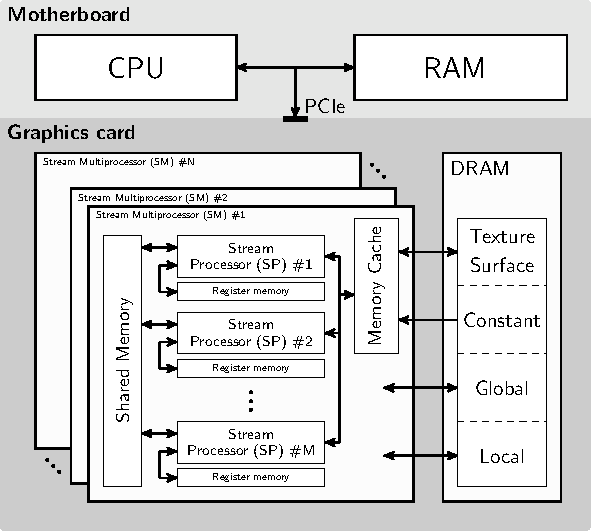
\includegraphics[width=\textwidth]{GPUmethods/architecture-figure0.pdf} 
\end{center}

\caption[Block diagram of a GPU architecture]{\label{fig:GPUarch} Diagram of a the basic architecture of a GPU. It shows how processing units and memory is structured inside a graphics card.} 
\end{figure}



The second part of the GPU are the memory types. There are 3 types of memory in the GPU: registers, shared memory and device random access memory (DRAM). The main difference between them is in accessibility (what subset of the SPs can access it) and speed. The lowest level memory is register memory. This is a thread level memory, used to store all local variables during execution. It is fast access and low in size. No other thread or block can access this memory. The second memory type is shared memory. This memory is used when blocks need to share information, such as the result of a computation in the middle of the kernel. Each SM has its own shared memory and it is local to them. All blocks can access to it, but careful usage of it is needed as the parallel nature of the computation could mean multiple writing on the same memory by different blocks. This memory is bigger (up to 48KB) and it is fast access, but slower than registers. Finally, there is DRAM memory. DRAM memory is a global large (12GB) memory on the board. This memory is widely used as it is the place where memory before kernel calls is allocated and where the results are stored after kernel calls. However, GPU code will often need to work with big data, thus the DRAM read/write is also commonly used within kernels. DRAM accessing can lead to significant bottlenecks as a single memory access needs 200 to 300 clock cycles to be carried. 

To improve memory throughput, the GPU contains so-called L1/L2 cache memory on each of the SMs. This cache is designed to improve execution of \textit{memory coalescing} warps. The cache, having a faster communication bus with the threads (needing about 80 cycles for a single memory read) stores a large amount of memory each time a single read to the DRAM is performed. The memory is loaded with locality, i.e., a memory chunk around the first sampled value is loaded, as the cache expects subsequent memory reads to be adjacent. Thus, when designing kernels, the order of the memory access can have a big influence on the final speed of the program. 

Two memory types can be used when data locality needs to be exploited in cache access: texture and surface memory. The difference between them is that the former is read only while the later can also be written. These memories can be defined as 3D shaped, thus data locality can be exploited in all spatial dimensions. Additionally, both can be accessed with floating point index values, and the memory value is returned with user-chosen interpolated methods. If cached memory is desired, but not in a spatially correlated form, then the read only constant memory can be used. This memory is still cached and can be used to speed up values that may be needed often. Then there is the global memory, which is read and write but not cached. Finally, local memory is an extension of shared memory when it gets filled.

The third important section is the communication between CPU-GPU. This is done via PCI-express ports and it is a slow communication process. Passing data from CPU to GPUs is relatively fast (500Mb/s), but can be a bottleneck in memory-heavy applications such as CT imaging.



\subsection{Exploiting GPGPUs for CT}

In CT, two main operations need to be accelerated: projection and backprojection. While iterative algorithms are defined as algebraic methods using a big system matrix $A$, the matrix itself is rarely used alone in the equations, it is generally used as $A*x$ or $A^T*b$. Fortunately, these two operations have a physical meaning, as the projection is the integral of the image over the straight X-ray paths, and the backprojection is the ``smearing'' of the detector data over the image back in the direction of the source, also following straight paths. While computing the values of the rows and columns of the system matrix seems hardly possible in real time, these two operations can be performed abstracting from their algebraic equivalent. The projection operation is an integration over independent, yet closely related, straight paths. By being able to sample the image domain in parallel, the operation can be performed at high speed. Similarly, the backprojection relies on building straight lines from the source to the voxels or detectors (dependent on the backprojection type), and sampling the projections. These operations are completely independent, hence the idea for GPU parallelism as threads will reach their maximum performance when they do not need to communicate with each other.  Additionally, both operations need accurate sampling over large volumes, thus texture memory with interpolation is ideal as it is hardware optimized, giving faster interpolated values than in a CPU or any possible interpolation kernel. Thus the massive parallelism and texture memory are they key features of GPU computing that make it the ideal tool for accelerating tomography. The following sections provide more details.

\section{The projection operator}
The projection operator is the numerical equivalent of the X-ray integral that defines the model of X-ray tomography (see equation XX). This operator models the idealized physics, where all the X-rays have an infinitely small width and travel in a straight path to the center of each detector pixel, and all with the same energy. While this may not represent the physics accurately enough to be a reliable X-ray  simulation tool, it is exactly what iterative methods need, the $A*x$ operation. 


There are several method to simulate forward projection, all of them easily parallelizable. One of these is the distance-driven projection \cite{BrunoDeMan}\cite{schlifske2016fast}, where the ray-voxel and detector intersections are all projected in a mid-plane and values are accumulated there. Alternatively, the voxel-driven projector\cite{Du2017}, where the whole voxel (square or other shape\cite{lewitt1992alternatives}) is projected onto the detector and its values spread among all the corresponding pixels. With a similar approach, the separable footprints technique\cite{long20103d}\cite{wu2011gpu} approximates the footprint of the voxel in the detector for speed-up.  According to the authors it is more accurate than the distance-driven projection and faster than both the voxel-driven and distance-driven ones. Finally, in ray-driven projection\cite{siddon1985fast}\cite{xu2010fast}\cite{chou2011fast} methods the line path is integrated. Among these, the most important variations worth mentioning are the infinitesimally small exact path, area path, and the grid-interpolated path. The exact path computes either the length of an infinitesimally narrow path or the area of a finite width path over each voxel and uses that as a weight for the integral. The grid-interpolated projector instead sets a fixed sample length and interpolates voxel values. According to a study by Fang and Mueller\cite{1625152}, the most accurate methods are the ray-driven ones.

This work has focused on the infinitesimally small ray-voxel intersection and grid-interpolated methods only because in both the desired accuracy and speed have been reached. The grid-interpolated method also is a key method for the following chapters (see Chapter 6 for more information). As the projection is basically an integral of a volume over thousands of independent paths, it is straightforward to parallelize by independently computing each ray. The ray-voxel intersection method is equivalent to the algebraic representation, where the $A$ matrix contains the length of the intersection between voxels and the path. Those are multiplied and added to the voxel values themselves to obtain the detector values. However, while not feasible in CPUs, the grid-interpolated method can use the practically free (i.e., very little time overhead) texture memory interpolation for speed-up in GPUs. The difference between the methods can be seen in figure \ref{fig:Amatrix}. 

\begin{figure}

\begin{center} 
\subfigure[]{ 
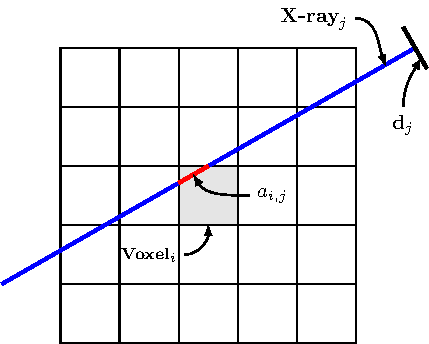
\includegraphics[width=0.45\linewidth]{GPUmethods/Amatrix-siddon.pdf} 
\label{fig:AmatrixSiddon} 
}
\subfigure[]{ 
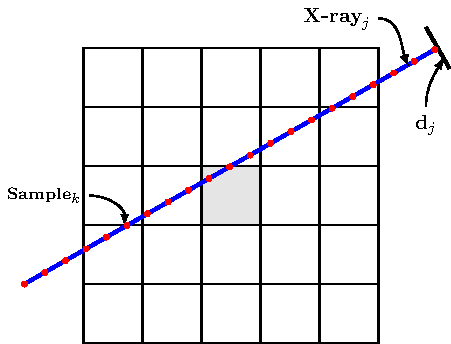
\includegraphics[width=0.45\linewidth]{GPUmethods/Amatrix-interp.pdf} 
\label{fig:AmatrixInterp} 
}
 
\caption[Diagram of projection types]{\label{fig:Amatrix}(a) Diagram of the projection operation using the line-voxel intersection methods and (b) diagram of the interpolated sampling method.} 
\end{center} 
\end{figure}

\FloatBarrier

\subsection{Ray-voxel intersection method}

As previously mentioned, this method relies on accumulating the length of the intersection between a straight path and voxels multiplied by the voxel value. The X-ray integral from equation XX can be discretized as in equation \ref{eq:ray-voxel}, where $d_{uv}$ is the detector value of X-ray $uv$, $\mathbb{I}(ijk)$ are the voxel values of the image and $l_{uv,ijk}$ the length of the path within each voxel. Note that here $l_{uv,ijk}$ are the same values as the elements of matrix $A$. Computing $l_{(uv,ijk)}$ requires some geometrical computations, not only the reliable detection of the intersections between the lines and voxel boundaries, but also avoiding computing it on voxels where the line does not intersect.

\begin{equation}
d_{(uv)}= \sum_{ijk=0}^{N_\mathbb{I}}l_{(uv,ijk)}*\mathbb{I}(ijk)
\label{eq:ray-voxel}
\end{equation}


\begin{figure}
\begin{center}

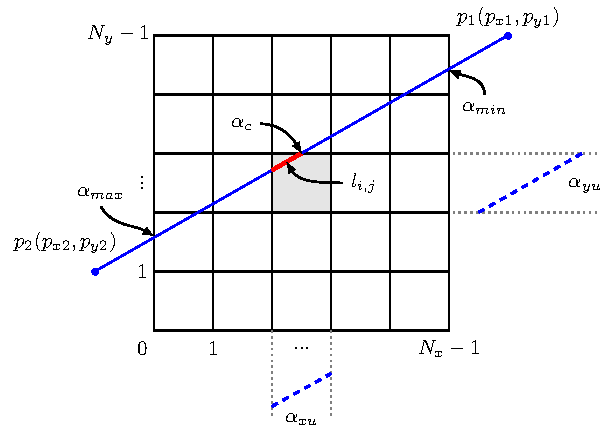
\includegraphics{GPUmethods/Amatrix_siddon_diagram.pdf} 
\end{center}

\caption[Jacob's ray tracing diagram]{\label{fig:Siddon} Diagram of the relevant variables for Jacobs' ray-tracing algorithm.} 
\end{figure}



The algorithm to compute $d_{uvj}$ has been taken from Jacobs\cite{jacobs1998fast} improvement on Siddon's method\cite{siddon1985fast}. For the sake of clarity, the algorithm is described for the 2D case, but the extension to 3D is trivial. The algorithm is based on computing the intersection between the path and the x and y planes and iterating over the ray until the next intersection is found. The diagram of the variables used in the algorithm can be seen in figure \ref{fig:Siddon}. The following derivation assumes that the pixels are of size 1 and the image domain starts at $(0,0)$, as this assumption reduces the number of operations needed. Assuming non-trivial rays from point $(p_{x1},p_{y1})$ to point $(p_{x2},p_{y2})$, the parametric representation of the ray is
\begin{equation}
p_{12}=
\begin{cases}
      p_x(\alpha)&=p_{x1}+\alpha (p_{x2}-p_{x1})\\
      p_y(\alpha)&=p_{y1}+\alpha (p_{y2}-p_{y1}),\label{eq:line}
    \end{cases}
\end{equation}
where $\alpha \in [0,1]$. In order to know the number of intersections, the initial and final intersections of the ray in the image are needed. The intersection points in terms of alpha can be defined as
\begin{equation}
\alpha_x(i) = \frac{(i-p_{x1})}{p_{x2}-p_{x1}}\label{eq:alphax}
\end{equation}
\begin{equation}
\alpha_y(j) = \frac{(j-p_{y1})}{p_{y2}-p_{y1}},\label{eq:alphay}
\end{equation}
where $i$ and $j$ are indices of the pixels. If the number of planes is defined as $N_x$ and $N_y$, one can compute the minimum and maximum $\alpha$ values (i.e., values of the line at the boundary of the image) by comparing the values of $\alpha$ in each direction as

\begin{align}
\alpha_{min}&=\max \Big(\min \big(\alpha_x(0),\alpha_x(N_x-1)  \big), \min \big(\alpha_y(0),\alpha_y(N_y-1)  \big) \Big)\\
\alpha_{max}&=\min \Big(\max \big(\alpha_x(0),\alpha_x(N_x-1)  \big), \max \big(\alpha_y(0),\alpha_y(N_y-1)  \big) \Big).
\end{align}
Note that this is equivalent to writing

\begin{align}
\alpha_{min}&=\max \Big( \alpha_{xmin},\alpha_{ymin} \Big)\\
\alpha_{max}&=\min \Big( \alpha_{xmax},\alpha_{ymax}\Big).
\end{align}

Next, the planes where the rays first cross in each direction need to be computed. This can be achieved by looking at the different $\alpha$ values. For the $x$ dimension, equations \ref{eq:alpha1-1}-\ref{eq:alpha1-2} show how to compute the plane index $i_{min}$ and $i_{max}$ if $p_{x1}<p_{x2}$ and equations \ref{eq:alpha2-1}-\ref{eq:alpha2-2} when $p_{x1}>p_{x2}$. The same logic applies to $j_{min}$ and $j_{max}$.

\begin{align}
\alpha_{min}&=\alpha_{xmin}\quad \rightarrow\quad i_{min}=1 \label{eq:alpha1-1}
\\
\alpha_{min}&\neq\alpha_{xmin}\quad \rightarrow\quad i_{min}=\lceil{ p_x(\alpha_{xmin})}\rceil \\
\alpha_{max}&=\alpha_{xmax}\quad \rightarrow\quad i_{max}=N_x-1\\
\alpha_{max}&\neq\alpha_{xmax}\quad \rightarrow\quad i_{max}=\lfloor{ p_x(\alpha_{xmax})}\rfloor 
\label{eq:alpha1-2}
\end{align}
\begin{align}
\alpha_{min}&=\alpha_{xmin}\quad \rightarrow\quad i_{max}=N_x-2 \label{eq:alpha2-1}\\
\alpha_{min}&\neq\alpha_{xmin}\quad \rightarrow\quad i_{max}=\lfloor{ p_x(\alpha_{xmin})}\rfloor \\
\alpha_{max}&=\alpha_{xmax} \quad\rightarrow\quad i_{min}=0\\
\alpha_{max}&\neq\alpha_{xmax} \quad\rightarrow\quad i_{max}=\lceil{ p_x(\alpha_{xmax})}\rceil .
\label{eq:alpha2-2}
\end{align}

At this point, the $\alpha_x$ and $\alpha_y$ values of the first intersection point can be obtained by substituting either $(i_{min},j_{min})$ or $(i_{max},j_{max})$ (depending on the relationship of $p_1$ and $p_2$) into equations \ref{eq:alphax} and \ref{eq:alphay}. Additionally, one can compute the number of planes that the ray crosses ($N_p$) with the following equation:
\begin{equation}
N_p=(i_{max}-i_{min}+1)+(j_{max}-j_{min}+1).
\end{equation}

In order to be able to start iterating over a given line there are just two pieces of information missing, namely the initial pixel coordinates and the $\alpha_u$, the maximum step in each direction for a unit of change. The initial pixel coordinates can be computed as

\begin{align}
i&=\bigg\lfloor{p_x\Big(\frac{min(\alpha_x,\alpha_y)+\alpha_{min}}{2}\Big)}\bigg\rfloor\\
j&=\bigg\lfloor{p_y\Big(\frac{min(\alpha_x,\alpha_y)+\alpha_{min}}{2}\Big)}\bigg\rfloor.
\end{align}

The maximum $\alpha$ that can happen in a unit of change in each direction, or $\alpha_{xu}$ and $\alpha_{yu}$ are defined as in equation \ref{eq:unitalpha}. Additionally it is useful to have a variable that controls the unit direction of the ray, $i_u$ and $j_u$, as in equation \ref{eq:direction}.

\begin{equation}
\alpha_{xu}=\frac{1}{\left|p_{x2}-p_{x1} \right|}\label{eq:unitalpha}
\end{equation}
\begin{equation}
i_u=
\begin{cases}
1 & \text{if}\quad p_{x1}< p_{x2}\\
-1 &\quad\quad\text{otherwise}
\end{cases}\label{eq:direction}
\end{equation}

Defining $l_{tot}$ as the Euclidean distance between $p_1$ and $p_2$ and initializing the current $\alpha$, $\alpha_c=\alpha_{min}$, the iterative method to follow the X-ray path can be described as follows. Check if the next intersection is in $x$ or $y$ by comparing the $\alpha$ values of each direction, then choose to update the direction that has a smallest $\alpha$. When updating, compute the length of the next distance and update the $\alpha$, pixel index and integral values. The update when $\alpha_x<\alpha_y$ can be seen in equations \ref{eq:siddonUpdatex1}-\ref{eq:siddonUpdatex2}, and the opposite case in equations  \ref{eq:siddonUpdatey1}-\ref{eq:siddonUpdatey2}.
\begin{align}
d_{ray}\quad&=\quad d_{ray}+(\alpha_x-\alpha_c)\cdot l_{tot} \cdot\mathbb{I}(i,j)\label{eq:siddonUpdatex1}\\
i\quad&=\quad i+i_u\\
\alpha_c\quad&=\quad\alpha_x\\
\alpha_x\quad&=\quad\alpha_x+\alpha_{xu}\label{eq:siddonUpdatex2}
\end{align}
\begin{align}
d_{ray}\quad&=\quad d_{ray}+(\alpha_y-\alpha_c)\cdot l_{tot}\cdot\mathbb{I}(i,j)\label{eq:siddonUpdatey1}\\
j\quad&=\quad j+j_u\\
\alpha_c\quad&=\quad\alpha_y\\
\alpha_y\quad&=\quad\alpha_y+\alpha_{yu}\label{eq:siddonUpdatey2}
\end{align}
This process is repeated $N_p$ times and, while there may be degenerate cases where a cross-section between an $x$ and $y$ plane is repeated, the algorithm will compute a length of zero the second time, thus resolving the situation without need of a check.




%% THIS in optimization section?


This algorithm is highly parallelizable. It needs no memory but for a few scalars and, once the values of the required variables are computed, the iterative process that takes most of the time is defined by 4 simple equations. A few straightforward optimizations are also possible, such as multiplying by $l_{tot}$ outside the for loop, in the end of the iterative process and precomputing the few scalar operands that are reused during the process to minimize the number of algebraic operations.




From the iterative section, the memory reads, $\mathbb{I}(i,j)$, are the most computationally expensive part. As previously commented, a single memory read takes 80 cycles as a best case, compared to just one for an algebraic operator involving two scalars. This is true for proper memory access. If the memory is accessed in a random manner, the memory latency increases massively. Thus making sure that single warps (32 simultaneous threads) read from memory in a similar matter is key. Additionally, \textit{thread divergence} can slow down the overall execution. Thread divergence refers to the case where, due to control flow such as a different path in an \textbf{if} condition, threads compute different things and finish at different times. If this happens, they will stay idle until the slowest threads are finished, effectively wasting time. In order to decrease memory latency, texture memory is used. One of the features of texture memory is that the cache will assume data locality, thus loading a chunk of memory around the sampled value. If threads read around it, then the memory reads are faster. In order to implement that, the X-rays are divided into divU$\times$ divV pieces, and launched in each block together, as seen in figure \ref{fig:block}. This ensures that the all rays are as close to each other as possible and hence that samples are taken next to each other. Interestingly, this approach also minimizes thread divergence, as X-rays very close to each other will cross each voxel boundary in a similar manner, and will most likely have the same $N_p$ number of intersections. It is important to note though that the figure oversimplifies the real case scenario. The concurrent memory reads are not happening in a parallel plane to the detector as, due to the cone angle, some paths are longer than others and some paths can intersect more voxels than others. However, if $divU\times divV$ is small enough, then this divergence is small enough that it has no effect on the computation time because the difference in the source-to-detector direction is still within the cached memory size.


\begin{figure}
\begin{center}

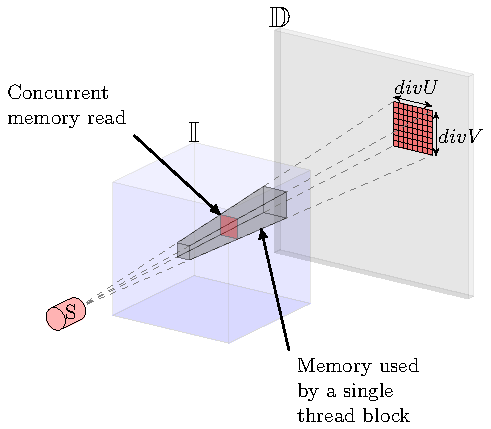
\includegraphics{GPUmethods/threadblocks-figure0.pdf} 
\end{center}

\caption[Diagram of trheadblock optimized kernel execution]{\label{fig:block} Diagram of the block level execution and memory access to increase data locality. Each block is composed of $divU\times divV$ rays, which are executed in parallel. This ensures that the concurrent memory reads are spatially adjacent, thus decreasing memory latency.} 
\end{figure}




\subsection{Grid-interpolated methods}

The grid-interpolated method is significantly less complex than the ray-voxel intersection method. As shown in figure \ref{fig:AmatrixInterp}, it merely relies on sampling the X-ray paths with a uniform Euclidean sampling rate. It can be described using equation \ref{eq:interpolated} and its pseudocode is given in \ref{alg:gridinterp}.

\begin{equation}
d_{(uv)}= \sum_{\alpha}\Delta l*\mathbb{I}(p_x(\alpha),p_y(\alpha),p_z(\alpha)),
\label{eq:interpolated}
\end{equation}
where $\alpha$ is the parameter of the line equation and takes decimal values between 0-1 if defined in terms of the source and detector locations (see equation \ref{eq:line}). Note that now the image $\mathbb{I}$ is sampled using not integer values, but decimal values, thus requiring interpolation. The texture memory cache includes hardware accelerated linear interpolation, so this is interpolation method used. Whereas in equation \ref{eq:ray-voxel} the length in this projection method, $\Delta l$, is a constant the same for all samples and thus can be taken out of the summation.

\begin{algorithm}

\caption{Grid interpolated projection
\label{alg:gridinterp}}
\begin{algorithmic}[1]
\State{Precompute geometric constants}
\Require{$N_{ray}$ threads organized in divU$\times$divV blocks}
    
\For{X-ray path}
      \State{Compute $[x_p,y_p,z_p]$ sample position}
      %\State{Sample $[\textup{DVF}_x,\textup{DVF}_y,\textup{DVF}_z]= \textup{DVF}(x,y,z)$}
      \State{Sum+= $ \textup{Image}(x_p,y_p,z_p)$}      
\EndFor
\State{Detector($u,v$)=$\Delta l \cdot Sum$}
\Ensure{} 
\end{algorithmic}

\end{algorithm}


The memory latency is significantly decreased by choosing the same structure for block and thread organizing as used in the other method and shown in figure \ref{fig:block}. The sampling rate of $\alpha$ is the relevant parameter to set and, as discussed by Jia \textit{et al}\cite{jia2012gpu}, it defaults to half the voxel size to ensure all data are used. The implementation in TIGRE additionally blocks the user from choosing a sampling rate larger than a voxel by limiting it to that size and changing the interpolation to nearest neighbour.

This method of projection is arguably more realistic than the ray-voxel projection in the case where the voxel size is very big (the resolution is very low) as it treats image information as a continuous domain instead of square boxes.

\subsection{Comments on optimization}

In order to minimize the computation times several optimization tricks have been used in both projection types. As one of the challenges of GPU programming is that often the only way of knowing how to accelerate code or what approach to use is intuition and testing, describing the optimization tricks and tests used for acceleration can be important. Three tricks that are worth mentioning are implemented, namely choosing an optimal coordinate system, precomputing geometric unit changes, and the way out of bounds memory is handled. Aside from these, other small tweaks can be found in the code, such as never computing trigonometric functions inside the kernels, but they are all relatively trivial and no further comment on them will be made.

\subsubsection{Optimal coordinate system}

When designing a kernel one of the main considerations is to minimize the amount of arithmetic operations happening inside. In tomography specifically, the geometry is the most variable of the parameters. Images can be arbitrarily fine or coarse and voxels can be anisotropic with a wide range of sizes in each direction and so can the detector. Thus, when writing the kernel, a coordinate system is needed that can accommodate the flexibility of the geometry while still being minimal in arithmetic operations. In TIGRE, the following has been chosen for the projector operator.

As the image memory is static, and data needs to be sampled from it in the projection coordinate system, the image will never move, while the detector and the source will rotate around the axis of rotation. Thus the new system ($x_p,y_p,z_p)$ is aligned with the image edges and it is centred at the first lexicographically indexed voxel, at the bottom corner of the image as seen in figure \ref{fig:projcoord}.  Additionally, the units of the new system are set as voxels, regardless of the size of the voxels in each direction. This new system reduces the amount of arithmetic operations as each sample point is now an index in the image memory, while in each kernel the vector from the source to the detector position must be computed arithmetically. Thus, in the main loop where the new sample location is needed, once the next point in the line is computed no more operations are needed to convert to memory index. This alone saves a significant time.


\subsubsection{Precomputation of geometry}

In order to generate the new coordinate system, some transformations need to be applied to the input geometry, as the units, source location and detector locations need to be set up. All these operations are performed outside the kernel and output 2 points and 2 vectors. The points are the location of the source and first detector pixel with respect to the new coordinate system origin, rotation angle and other geometric definitions. The vectors describe the unit change in projection coordinate systems of the detector pixel location, thus by knowing the location of the first detector pixel and their unit changes, finding any detector pixel location from its index is trivial.

Additionally, the advantage of structuring the geometry computations as described is that new geometric transformations can be implemented with zero increase in computational cost. For example, the addition of the rotation with 3 degrees of freedom of the detector, offset of the image with respect to the axis of rotation or offset of the detector implies no change in computational cost, the only change needed is the change in the 2 points and vectors described.
 
 % sampling outside the image
\subsubsection{Sampling outside the image}

In the ray-voxel method, sampling outside the image is not a worry as the amount of cross-sections and the initial intersection are computed in the algorithm. However, in the grid-interpolated method, a start and end point for sampling need to be chosen. 

As the texture memory is cached and handled differently than a direct read into memory, it has multiple tunable features. One of these is the possibility of selecting the behaviour when a memory read is out of bounds, which in the case of this work is set to zero. It is important to note that this means the code will not generate an error for out of bounds memory reads. Two versions of the grid-interpolated method can be tested, one where there is a conditional check to see if the current point is inside the image and if true then sample, and another where the line is sampled from the source to the detector. Empirical tests show that avoiding the conditional statement and sampling over the whole path is 33\% faster than checking if the sample is within bounds, even with geometry definitions where more than 50\% of the samples lie outside the image. This can be explained by the fact that CUDA cores are quite slow with code control flow and possibly\footnote{This is undocumented so, while it is very likely, it is hard to claim with full certainty.} by the cache taking virtually no time returning a zero value when accessed out of bounds. 

% explain min max radius for out of bounds
Sampling the x-ray path from the start to the end is not optimal either, even avoiding conditional statements. To minimize the memory reads, the diameter of a cylinder that encloses the image is precomputed and the rays are sampled from the beginning of the cylinder to either the detector or to the end of the cylinder, whichever comes first. This approach speeds the projection kernel by another 20\%. This is shown in figure \ref{fig:projcoord}.

\begin{figure}
\begin{center}

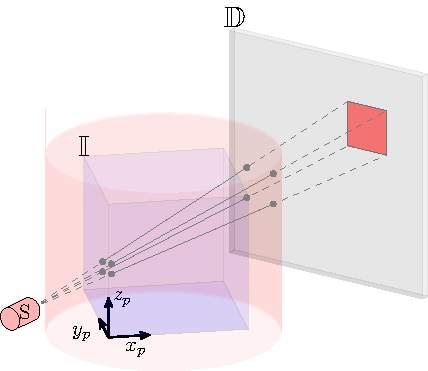
\includegraphics{GPUmethods/projcoord-figure0.pdf} 
\end{center}

\caption[Projection coordinate system]{\label{fig:projcoord} Diagram of the projection coordinate system and sampling region. In both projection operations the new coordinate system ($(x_p,y_p,z_p)$) has its origin on the lexicographically first voxel center. The red cylinder shows the sampling region for the grid-interpolated method, where the kernels sample from memory.} 
\end{figure}
\subsection{Differences between operators}

The projection operators, while effectively simulating the same physics, have slightly different results due to the methods used. The difference between the two projection operators is enhanced when the voxel size of the images is very big, i.e., when the image has low resolution. Figure \ref{fig:projtypes} shows this effect. A projection of the 3D Shepp-Logan phantom is shown at different resolutions for both projection types. In the figure, four image resolutions can be seen for the same size, $64^3$, $128^3$, $256^3$ and $512^3$ from top to bottom. From left to right the first two columns show the ray-voxel intersection and the grid-interpolated method, while the last two columns show a zoomed in version of the same projections. Figure \ref{fig:projtypesdiff} shows the differences between the projections.

The ray-voxel intersection method does introduce higher aliasing-like artefacts to the projection, as opposed to the interpolating method that smooths everything. Note however that when the image resolution gets higher, the differences are almost indistinguishable. None of the projection modes is better or worse. One could argue that the ray-voxel method aligns better with the discretization of the domain, or that the interpolated method is better because it generates images that are closer to what is measured in a real detector. 


When used in reconstruction, the differences between the images reconstructed with algorithms using one or the other projection types are insignificant, with generally a maximum value of about 0.1\% of the highest value in the image. This can be seen in figure \ref{fig:OSSART200proj}, where a reconstruction of the XCAT\cite{XCAT} phantom of size $256^3$ using OS-SART with 200 iterations and 100 projections is shown. It shows the result using both projection operators, and figure \ref{fig:OSSART200projdiff} the contrast enhanced differences (the colourmap is enhanced to 10\% of the maximum data value) of both reconstructions against the original image. Both reconstructed images are visually very similar and the enhanced difference images show structural differences in the error, but they are still of the same level. The sum of square errors shows a slight higher value for the ray-voxel method, but not big enough to be significant. This difference is even smaller when working with higher resolution images. TIGRE defaults to the interpolated projection in the algorithms.

% RMSE= 3.18 vs 2.73


\begin{figure}
\centering
\begin{tikzpicture}

\node (A) {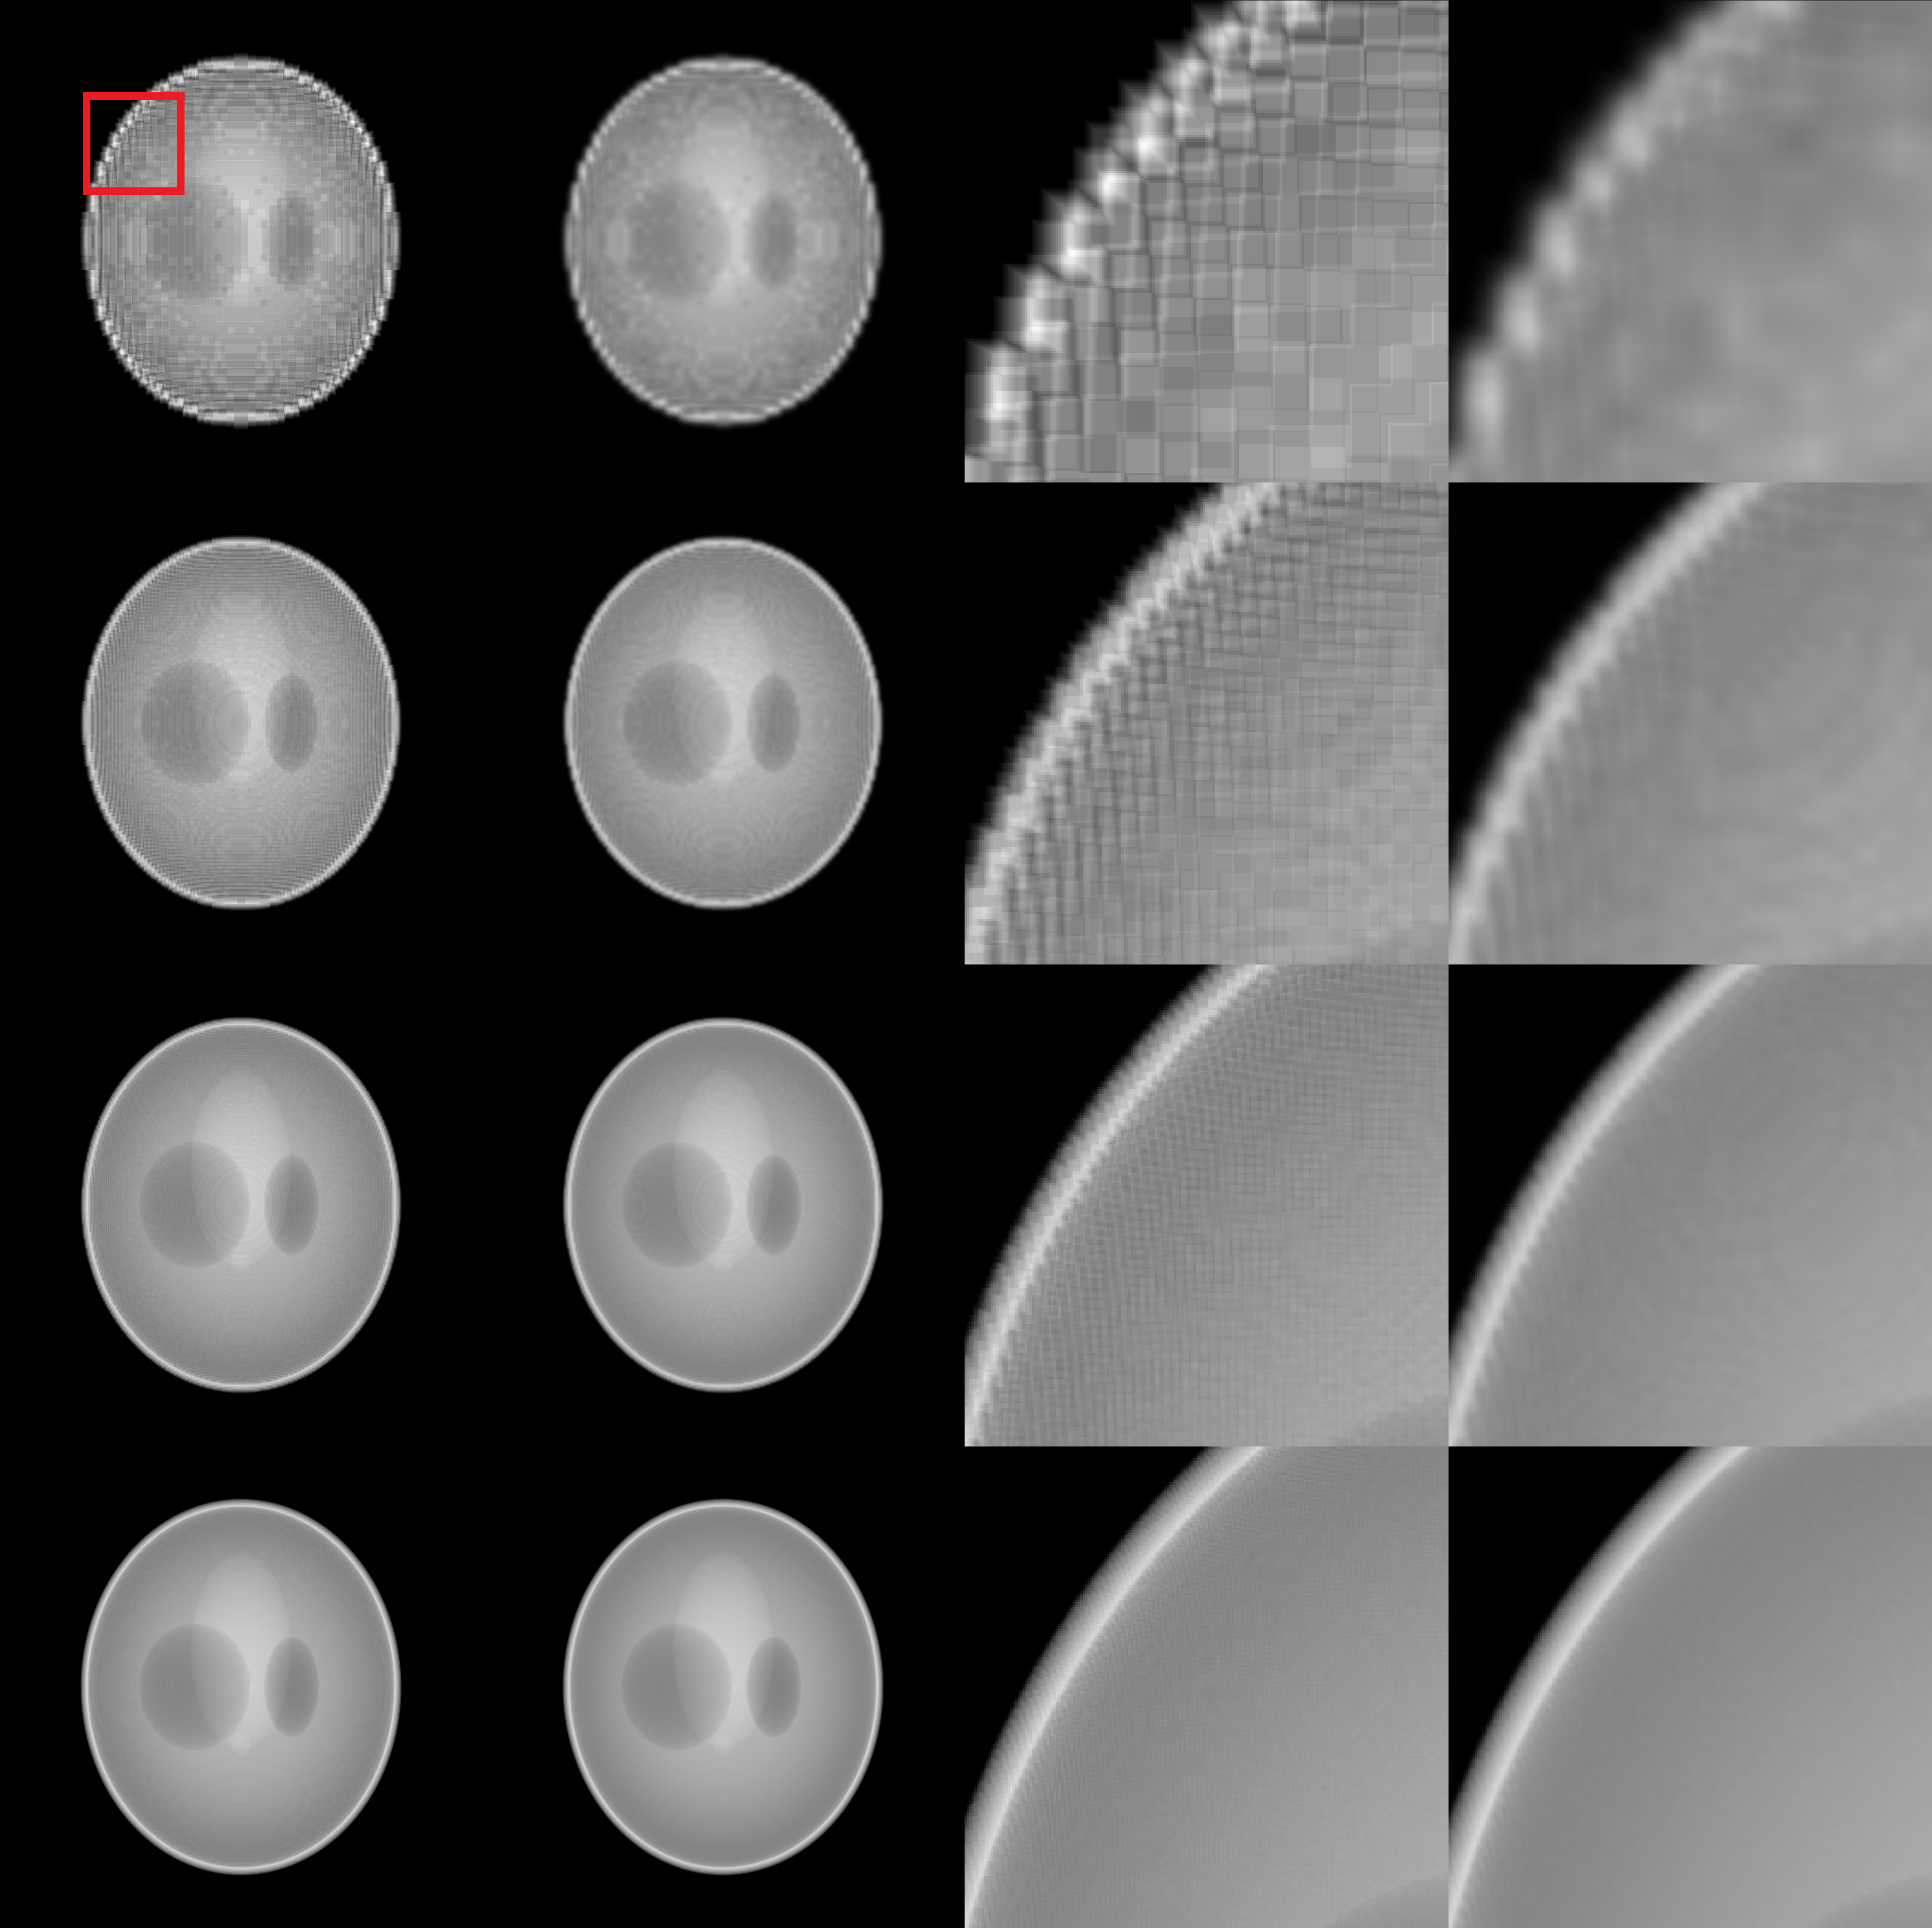
\includegraphics[width=0.94\textwidth]{GPUmethods/projtypes.png} };
\path (A.south west) -- (A.north west) node[pos=.125, above, rotate=90] {$512^3$} node[pos=.375, above, rotate=90] {$256^3$} node[pos=.625, above, rotate=90] {$128^3$} node[pos=.875, above, rotate=90] {$64^3$};
\path (A.south west) -- (A.south east) node[pos=.125, below] {(a)} node[pos=.375, below] {(b)} node[pos=.625, below] {(c)} node[pos=.875, below] {(d)};

\end{tikzpicture}

\caption[Comparison between projection operations]{\label{fig:projtypes} Different projection modes for different image resolutions. From top to bottom, the image resolution is $64^3$, $128^3$, $256^3$ and $512^3$ respectively. From left to right, (a) the ray-voxel intersection projection; (b) the grid-interpolated projection; (c) a zoomed in version of (a); and (d) a zoomed in version of (b).} 
\end{figure}

\begin{figure}

\centering
\begin{tikzpicture}

\node (A) {\includegraphics[width=0.94\textwidth]{GPUmethods/projtypesdiff.png} };
\path (A.south west) -- (A.north west) node[pos=.125, above, rotate=90] {$512^3$} node[pos=.375, above, rotate=90] {$256^3$} node[pos=.625, above, rotate=90] {$128^3$} node[pos=.875, above, rotate=90] {$64^3$};
\path (A.south west) -- (A.south east) node[pos=.125, below] {(a)} node[pos=.375, below] {(b)} node[pos=.625, below] {(c)} node[pos=.875, below] {(d)};

\end{tikzpicture}
\caption[Difference between projection operations]{\label{fig:projtypesdiff} Difference between projection modes for different image resolutions. From top to bottom, the image resolution is $64^3$, $128^3$, $256^3$ and $512^3$ respectively. From left to right, (a) the absolute difference between the projections; (b) contrast enhanced version of (a) by cropping the colourmap to 25\% of the maximum; (c) a zoomed in version of (a); and (d) a zoomed in version of (b).} 
\end{figure}


\begin{figure}
\centering
\begin{tikzpicture}

\node (A) {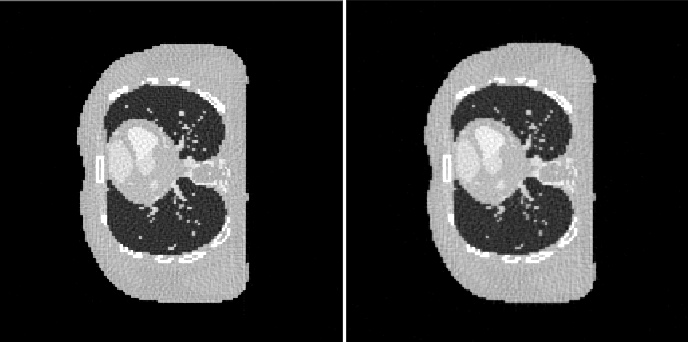
\includegraphics[width=0.98\textwidth]{GPUmethods/OSSART200.png} };
\path (A.south west) -- (A.south east) node[pos=.25, below] {(a)} node[pos=.75, below] {(b)};
\end{tikzpicture}

\caption[Reconstruction example using different projection operators]{\label{fig:OSSART200proj} XCAT phantom reconstruction of size $256^3$ using OS-SART with 200 iterations and 100 angularly uniformly sampled projections. (a) Reconstruction using ray-voxel intersection projection and (b) using the interpolated-projection method.} 
\end{figure}


\begin{figure}
\centering
\begin{tikzpicture}

\node (A) {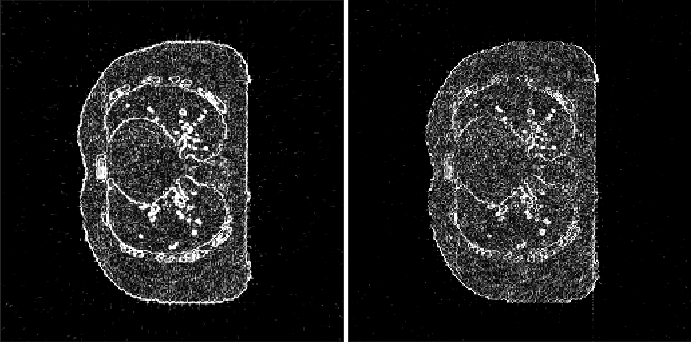
\includegraphics[width=0.98\textwidth]{GPUmethods/OSSART200diff.png} };
\path (A.south west) -- (A.south east) node[pos=.25, below] {(a)} node[pos=.75, below] {(b)};
\end{tikzpicture}

\caption[Difference in reconstruction using different projection operators]{\label{fig:OSSART200projdiff} Difference between the original XCAT phantom and the reconstructions of figure \ref{fig:OSSART200proj}. The colour limits have been set to 10\% of the maximum intensity of the original data.  (a) Difference using ray-voxel intersection projection and (b) difference with the interpolated projection method.} 
\end{figure}



\FloatBarrier

\section{The backprojection operator}

The backprojection operator (or $A^T*b$ in algebraic notation) is the operator that updates the image using the information in the projection images. This update is performed by an operation often described in the literature as a smearing of the projection data into the image, as if it were butter on toast, but following the path from detector to source.

As with projection, multiple methods to perform this operation have been proposed in the literature. The most commonly used method is voxel-driven backprojection\cite{scherl2007fast}\cite{okitsu2010high}, where the path from the source to each voxel center is generated and extended until the detector is reached. Then the value in the detector is sampled (using interpolation, as it is likely that it does not fall in the center of a pixel) and the voxel value updated.
 
Other methods include the separable footprints method\cite{long20103d}, where the footprint of the voxel in the detector is precomputed and approximated and the voxel values are updated according to the detector values overlapping the voxel footprint. A conceptually similar backprojection relies on having spherical shaped image value representation, instead of square voxels\cite{spherical}. The backprojection using basis-functions also updates the image values according to the footprint of these spherical voxels.
 
The distance-driven method\cite{schlifske2016fast} is also applicable to backprojection by performing the same operation as for projection: the computation of all voxel-pixel intersections in an imaginary mid-plane. Finally, ray-voxel intersection driven methods also exist\cite{park2015fully}, in both single ray or multiple ray per voxel modes. This method requires multiple voxel updates per backprojection, but can give a matched result, i.e., the backprojection method is the same as the projection method. This has been shown to give better results\cite{6829349} and allows the use of any iterative method Krylov subspace methods require matched backprojection. 
 
In this work, voxel-driven backprojection has been implemented. The rationale being that it is a method which is fast and easy to implement yet accurate. Additionally, a quasi-matched backprojection can be implemented to allow Krylov subspace algorithms (see section \ref{sec:weights} for more information). Finally, this method is most appropriate for the method proposed in Chapter 6.
 

\subsection{Voxel-driven backprojection}

The underlying idea of voxel-driven backprojection is simple, the path between the source and the center of each voxel is computed and the intersection of that path with the detector is computed. Then, the detector is sampled at the intersection point (using interpolation) and the voxel is updated with that value. Due to the cone angle, a weighting factor is also applied to each voxel (more details are given in the next section).

\begin{figure}
\begin{center}

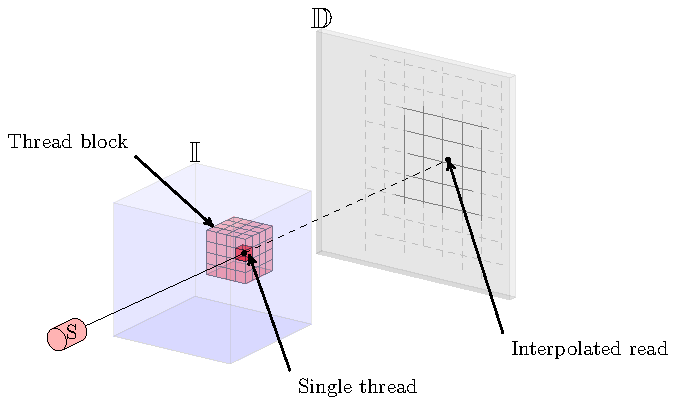
\includegraphics{GPUmethods/simplebackproj-figure0.pdf} 
\end{center}

\caption[Diagram of the voxel driven backproejction]{\label{fig:simpleback} Simple voxel-driven backprojection. Each kernel is subdivided into square blocks and each thread updates a single voxel using interpolated memory reads in the detector.} 
\end{figure}


To accelerate this operator in a GPU, the naive approach is to assign a thread per voxel and to assign a square amount of threads to a single block (by dividing it into divX$\times$divY$\times$divZ threads) to maximize cache hits on texture memory (used for the interpolation of the detector values). The block size is empirically set to 8x8x8 for fastest execution. This approach, shown as a diagran in figure \ref{fig:simpleback} and as pseudocode in algorithm \ref{alg:naiveback}, does indeed result in a fast kernel. However, the backprojection requires a significantly higher total number of threads than the projection operation, while repeating the same thing for each voxel (in multiple bakcprojection updates) and reading in the same memory very often. In order to improve the cache memory hits and minimize redundant arithmetic computations, a series of improvements have been studied by Papenhausen \emph{et al}\cite{papenhausen2011gpu} and further optimized by Zinsser \emph{et al} \cite{zinsser2013systematic}.

\begin{algorithm}

\caption{Naive voxel-driven backprojection
\label{alg:naiveback}}
\begin{algorithmic}[1]
\For{Projection}
\State{Precompute geometric constants}


\Require{$N_{voxel}$ threads organized in divX$\times$divY$\times$divZ blocks}
      \State{\qquad Compute $[u,v]$ sample position}
      %\State{Sample $[\textup{DVF}_x,\textup{DVF}_y,\textup{DVF}_z]= \textup{DVF}(x,y,z)$}
      \State{\qquad Compute $w$ weight}
\State{\qquad Image($x,y,z$)+=$w  \cdot \textup{Detector}(u,v)$}
\Ensure{} 
\EndFor

\end{algorithmic}

\end{algorithm}


The main idea behind the optimization is the minimization of memory latency. In order to do that a multiple voxel, multiple projection per thread kernel is designed. If in each of the threads when a single voxel is updated multiple projections (32 in this case) are used, these will be spatially nearby, thus the L2 cache will speed up the memory reading process provided the angular distance between projections is small. Additionally, if each of the threads computes a small subset of voxels ($N_{voxelThread}$) in the $z$ direction (8 in this case), not only are the memory cache hits are likely to be increased, but also the computational operations reduced as the computation of the location of each voxel requires fewer operations. In general these tweaks increase the occupancy of the SMs, decreasing the amount of time the threads stand idle waiting for memory. The diagram of the new optimized kernel is shown in figure \ref{fig:optback} and its pseudocode is given in algorithm \ref{alg:optimizedback}. The code is divided in pieces to allow each block to have divX$\times$divY threads each (16$\times$32 in this case). To minimize global memory reads, the image voxel values that are updated in each kernel are pre-loaded. Then, for each projection, the geometric constants that describe the location of the detector and image pixels are loaded from constant memory. Next, the backprojection is performed for each voxel being updated. This approach further increases occupancy as in execution the thread does not wait for the memory read to finish before computing the next loop, thus hiding memory latency even more. Finally, the image is updated with the auxiliary variable. This step also decreases the memory latency, as fewer global memory write operations are needed.
% describe better the algorithm


\begin{algorithm}

\caption{Optimized voxel-driven backprojection
\label{alg:optimizedback}}
\begin{algorithmic}[1]
\For{$N_{kernels}$}
\State{Precompute geometric constants \textit{per projection}}

\Require{divX$\times$divY threads organized in $\frac{N_x}{\textup{divX}} \times \frac{N_y}{\textup{divY}} \times \frac{Nz}{N_{voxelThread}}$ blocks}
\For{$N_{voxelThread}$}
\State auxImage(voxThread)=Image($x,y,z$)
\EndFor  
\For{Projections (in this kernel)}
\State{Load geometric constants for this projection}
\For{$N_{voxThread}$}
\State{Compute $[u,v]$ sample position}
\State{Compute $w$ weight}
\State{auxImage(voxThread)+=$w  \cdot \textup{Detector}(u,v)$}
\EndFor
\EndFor
\For{$N_{voxThread}$}
\State{Image($x,y,z$)=auxImage(voxThread)}
\EndFor
\Ensure{} 
\EndFor

\end{algorithmic}

\end{algorithm}
\begin{figure}
\begin{center}

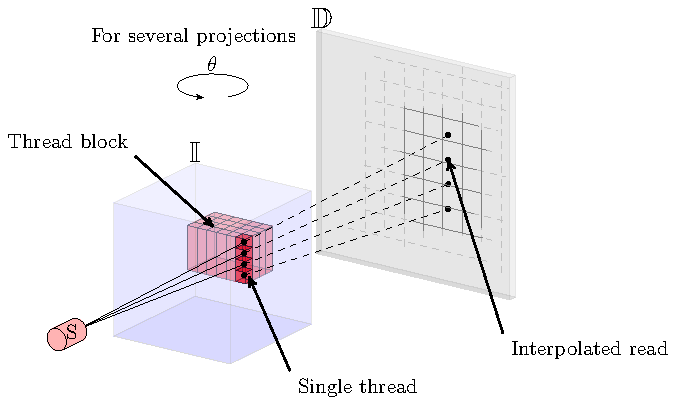
\includegraphics{GPUmethods/optbackproj-figure0.pdf} 
\end{center}

\caption[Diagram of multiple-voxel, multilpe-angle backprojection]{\label{fig:optback} Optimized voxel-driven backprojection. Each kernel is subdivided into blocks and each thread updates a series of vertical voxels using interpolated memory. Each kernel additionally operates in a series of projections, not in a single one.} 
\end{figure}

\subsection{Backprojection weights}\label{sec:weights}

Due to the cone shape the backprojection needs a weight for each voxel, as different paths have different ray lengths and hence have a different effect in the detector. In the projection operator, the length of the path is used in each detector pixel as a weight for the update, but in the backprojection operation the weight is not as straightforward to compute. In the algebraic definition of iterative algorithms, the weight of each voxel is the length of a specific ray within that voxel. If the matrices were fully known, it would be straightforward to compute (as it is the sum of the columns of $A$), however this doesn't apply to voxel-driven backprojection. In the GPU version, a projection to compute such lengths per backprojection would be needed, ultimately slowing the code considerably.

\subsubsection*{FDK weights}
A simple approach is to use the weights of the FDK algorithm as backprojection weights. As described in section XX, the FDK backprojection weight is computed as

\begin{equation}
w_{x,y}=\frac{R^2}{(R+y\cdot \sin\theta-x\cdot\cos\theta)^2},
\end{equation}
where $R$ is the distance from the source to the axis of rotation, $\theta$ the projection angle and $x$ and $y$ the location of the voxel. Note how this equation is independent of $z$, thus the weights can be precomputed after line 7 (instead of line 10) in algorithm \ref{alg:optimizedback}, resulting in a minor speed-up.


\subsubsection*{Pseudo-matched weights}
The FDK weights are good in the iterative algorithms that normalize the result of the backprojection afterwards (such as SART), as the overall scale and effect of the backprojections is removed in the algorithm by an opposing weighting factor. However, some algorithms require matched backprokection, i.e., a backprojection operator that is mathematically equivalent to the adjoint of the projection operator. This is not the case with FDK weights. Algorithms such as CGLS cannot work unless a matched backprojection is implemented. As previously explained, a fully matched backprojection, while possible, would slow down the kernels considerably due to the need of also computing projection operations in the backprojection. However Jia \textit{et al}\cite{jia2011gpu} propose a weight to match the backprojection.

In order to derive the weight, a functional analysis approach needs to be taken. For the sake of simplicity and cohesion with Jia \textit{et al}, the notation in this section differs from the rest of the thesis. 

If an image is represented as a function $f(\textbf{x})$, where $\textbf{x}=(x,y,z)\in \mathbb{R}^3$, a projection operator $A^\theta$ maps $f(\textbf{x})$ onto a different function on the projection plane with angle $\theta$ as:
\begin{equation}
A^\theta[f](\textbf{u})=\int_0^{L(\textbf{u})}\mathrm{d}l \ f(\textbf{x}_s+\textbf{n}l),
\label{eq:functionalXray}
\end{equation}
where $\textbf{x}_s$ is the coordinate of the source, $\textbf{n}$ a unit vector in the projection direction and $\textbf{u}\in \mathbb{R}^2 $ the coordinates in the detector. $L(\textbf{u})$ is the length of the X-ray path. 

Let $f(.):\mathbb{R}^3 \rightarrow \mathbb{R}$ and $g(.):\mathbb{R}^2 \rightarrow \mathbb{R}$ be smooth enough functions in image and  projection domain respectively. In order to to have an operator $A^{\theta^T}$ that is the adjoint of $A^\theta$, it should satisfy the condition 

\begin{equation}
\langle f, A^{\theta^T} g\rangle = \langle A^\theta f,g \rangle,
\end{equation}
where $\langle \cdot, \cdot\rangle $ is the inner product. In integral form, this inner product equality can be expressed as
\begin{equation}
\int \mathrm{d}\textbf{x}f(\textbf{x})A^{\theta^T} [g](\textbf{x})=\int \mathrm{d}\textbf{u}A^{\theta} [f](\textbf{u}) g(\textbf{u}),
\end{equation}
or if the functional derivative of both sides with respect to $f(\textbf{x})$ is taken, then as
\begin{equation}
A^{\theta^T} [g](\textbf{x})=\frac{\partial}{\partial f(\textbf{x})}\int \mathrm{d}\textbf{u}A^{\theta} [f](\textbf{u}) g(\textbf{u}).
\label{eq:matchedback3}
\end{equation}
Equation \ref{eq:matchedback3} can be rewritten as
\begin{equation}
A^{\theta^T} [g](\textbf{x})=\int \mathrm{d}\textbf{u}g(\textbf{u})\frac{\partial}{\partial f(\textbf{x})}A^{\theta} [f](\textbf{u}),
\label{eq:matchedback4}
\end{equation}
and equation \ref{eq:functionalXray} can be rewritten as equation \ref{eq:functionalXraydelta} using a delta function.
\begin{equation}
A^\theta[f](\textbf{u})=\int\mathrm{d}l\mathrm{d}\textbf{x} \ f(\textbf{x})\delta(\textbf{x}-\textbf{x}_s-\textbf{n}l).
\label{eq:functionalXraydelta}
\end{equation}

Finally, by substituting equation \ref{eq:functionalXraydelta} in \ref{eq:matchedback4}, the adjoint of the projection operator can be expressed as

\begin{equation}
A^{\theta^T}[g](\textbf{x})=\int\mathrm{d}l\mathrm{d}\textbf{u} \ g(\textbf{u})\delta(\textbf{x}-\textbf{x}_s-\textbf{n}l)=\frac{L^3(\textbf{u}^*)}{L_0l^2(\textbf{x})}g(\textbf{u}^*),
\end{equation}
where $\textbf{u}^*$ is the intersection point between the x-ray path and the detector plane, $l(\textbf{x})$ the distance between the source and a voxel, and $L_0$ the source to detector distance. This equation, however, applies to the integral form of the description of the system, while ultimately in the computer the matrix form is used. By changing the inner product to a vector form, the final adjoint over all projections becomes
\begin{equation}
A^{\theta^T}[g](\textbf{x})=\frac{\Delta x \Delta y \Delta z}{\Delta u \Delta v}\sum_\theta\frac{L^3(\textbf{u}^*)}{L_0l^2(\textbf{x})}g^\theta(\textbf{u}^*),\label{eq:finalmatched}
\end{equation}
where $(\Delta x,\Delta y,\Delta z)$ are the sizes of each voxel in each direction and $(\Delta u,\Delta v)$ the sizes of the detector pixels. 

This backprojector weight is very close to a matched backprojection operator. According to Jia \textit{et al} the numerical errors are less than 1\%. This work did not replicate their results. This mismatch can lead to inaccuracies in Hounsfield units in the final reconstruction and to divergent behaviour in the Krylov subspace algorithms, but only in late iterations.

\subsection{Comments on optimization}

To have a fast execution of the code, as for the projection, a geometry that minimizes the amount of arithmetic operations inside the kernels is proposed. The backprojection coordinate system $(x_b,y_b,z_b)$ is defined to have unit sizes of the detector pixel size in $u,v$ for $y_b$ and $z_b$ respectively, and 1mm in $x_b$. The origin of the system is located in the center of the first lexicographically ordered pixel in the detector and is always aligned to the detector (i.e., the image rotates while the detector-source system stays in the same location).  All precomputing operations performed in the projection geometry are also performed in here.

In the CUDA sense, two extra optimizations have been performed. By defining divX, divY and $N_{voxelThread}$ (from algorithm \ref{alg:optimizedback}) as compilers, an instruction to the CUDA compiler can be passed to unroll all the loops. Loop unrolling refers to replacing a for loop by a repetition of each line of code per iteration, one after the other. By doing this, the kernel does not need to have flow control (loop iteration, condition, variable) that needs increasing and checking, thus increasing the total kernel performance by 20\% in our case. A small speed-up is also obtained by defining the texture memory as layered memory, thus disabling interpolation in the third dimension.


\FloatBarrier
\section{Benchmark}\label{sec:speed}

This section shows the computational times for the projection and backprojection kernels. This section does test the performance of the kernels themselves, but the actual calls to the kernels do have some overhead of memory input and output, as it is a significant amount of memory that needs to be moved in every call. All computational time results show time per projection, for different image and projection sizes. Figure \ref{fig:projectiontimes} shows the projection times in milliseconds for both ray-voxel intersection and grid interpolated projection modes. The projection operation is dependent in both detector an image size, and it takes about the same time for both types of projection, with  maximum of 100ms with $1024^2$ detector and $1024^3$ image.


 Figure \ref{fig:backprojectiontimes} shows the backprojection times for FDK weights and pseudo-matched weights. As the kernels are optimized for adjacent projection calls the computational times do not scale with more projections, a test using the maximum projections per kernel is also performed. Figure \ref{fig:backprojection32times} shows kernel times per projection when multiple projections are updated. The maximum computational time on these tests ($1024^2$ detector with $1024^3$ image) show 75ms and 180ms for the FDK and pseudo-matched weights when a single projection is used, but 45ms and 99ms per projection when 32 projections (maximum simultaneously used projections in a single kernel) are used. Note that generally the pseudo-matched weights are slower. This is explained by the fact that the chosen kernel structure completely masks the memory latency with FDK weights, but with matched weights the arithmetic operations for the weight need both more computations and registers, thus slowing down the kernel significantly. Additionally an extra multiplication kernel is needed for the final normalization from equation \ref{eq:finalmatched}. Note also how the backprojection times are not dependant on the projection size, only in the image size. This is not a big surprise, considering how the kernels are designed.
 
 

 \color{black}{}
\begin{figure}
\centering
\begin{tikzpicture}
\node (A) {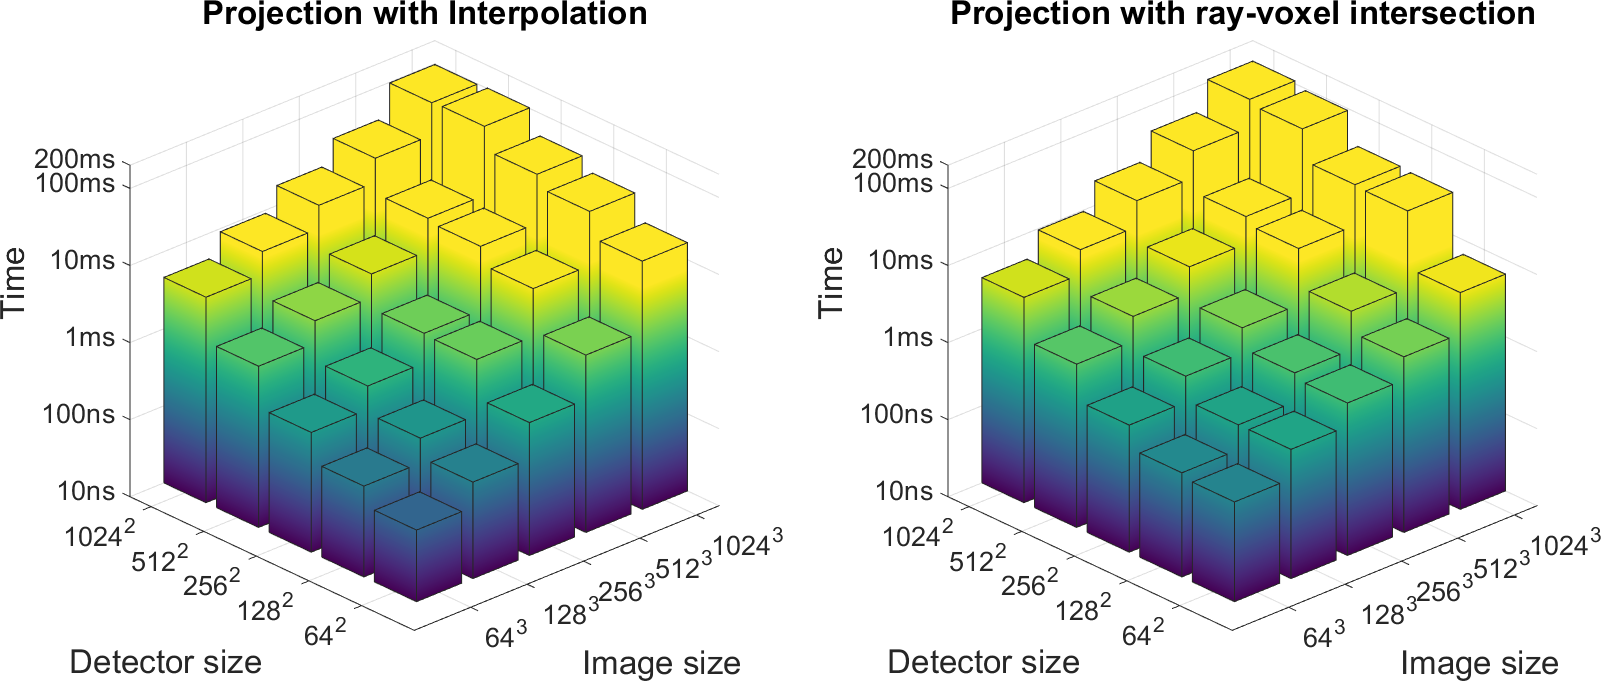
\includegraphics[width=0.98\textwidth]{GPUmethods/projection.png}};
\path (A.south west) -- (A.south east) node[pos=.25, below] {(a)} node[pos=.75, below] {(b)};
\end{tikzpicture}

\caption[Computational times of the projection operators]{\label{fig:projectiontimes} Computational times per projection for the projection operation for (a) grid interpolated (2 samples per voxel) and (b) ray-voxel intersection modes.} 
\end{figure}


\begin{figure}
\centering
\begin{tikzpicture}
\node (A) {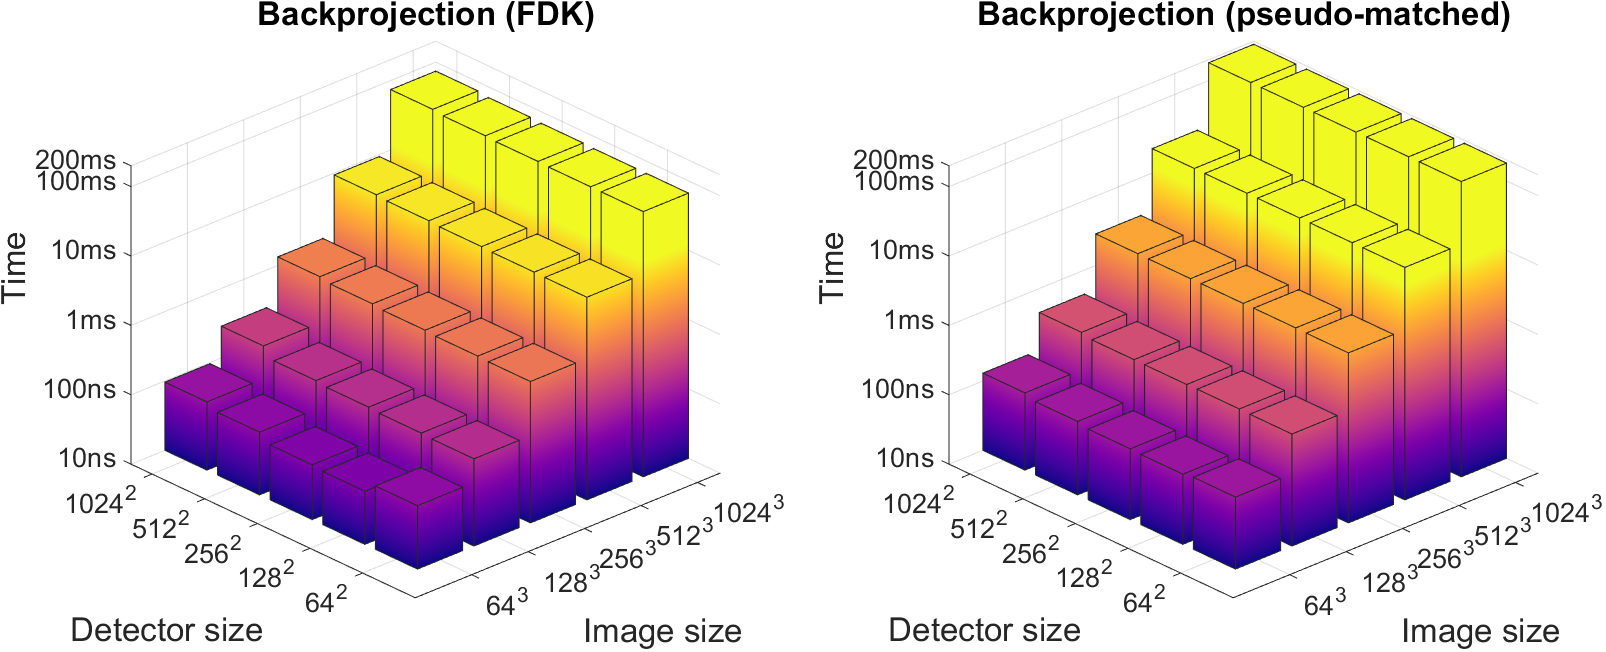
\includegraphics[width=0.98\textwidth]{GPUmethods/backprojection.png}};
\path (A.south west) -- (A.south east) node[pos=.25, below] {(a)} node[pos=.75, below] {(b)};
\end{tikzpicture}

\caption[Computational times of the backprojection operator, per projection]{\label{fig:backprojectiontimes} Computational times per projection for the backprojection operation when launched with a single projections for (a) FDK weights and (b) pseudo-matched weights.} 
\end{figure}

\begin{figure}
\centering
\begin{tikzpicture}
\node (A) {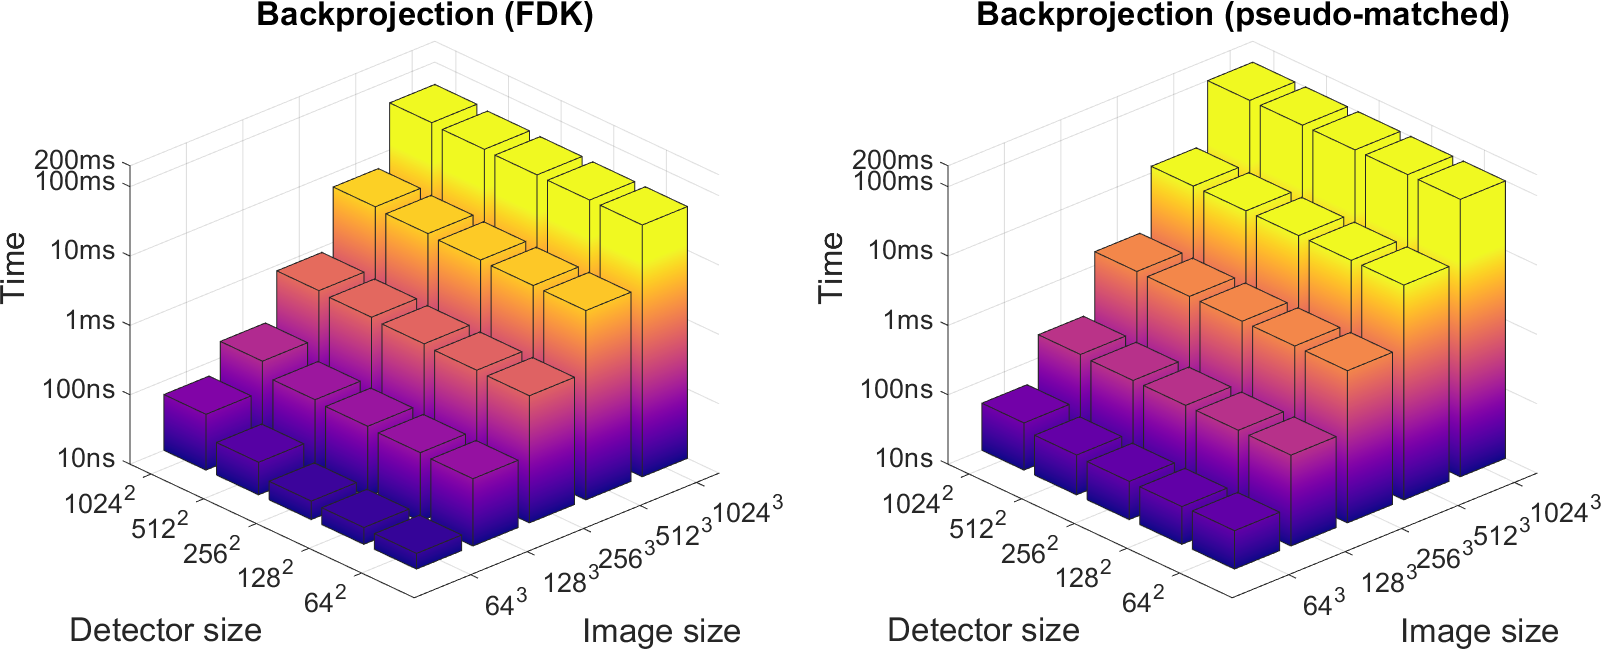
\includegraphics[width=0.98\textwidth]{GPUmethods/backprojection32.png}};
\path (A.south west) -- (A.south east) node[pos=.25, below] {(a)} node[pos=.75, below] {(b)};
\end{tikzpicture}

\caption[Computational times of the backprojection operator, multiple projections]{\label{fig:backprojection32times} Computational times per projection for the backprojection operation when launched with 32 projections for (a) FDK weights and (b) pseudo-matched weights.} 
\end{figure}


\FloatBarrier
\section{The TIGRE toolbox}

In order to have an easy tool to implement algorithms but still have the GPU acceleration on hand, a MATLAB-CUDA toolbox has been created, the Tomographic Iterative GPU-based Reconstruction toolbox, or TIGRE toolbox. TIGRE is a modular, easy to use fast toolbox for cone and parallel beam computed tomography, focusing in the implementation of a variety of iterative reconstruction algorithms. All four families of algorithms described in chapter 3 are implemented in TIGRE, namely, FDK, statistical inversion (MLEM), the gradient descend family (SART,OS-SART,SIRT), Krylov subspace family (CGLS) and TV regularized family (\mbox{ASD-POCS},  \mbox{OS-ASD-POCS}, \mbox{B-ASD-POCS-$\beta$}, SART-TV). This section describes the features of TIGRE, the geometry supported, the general structure of the toolbox and how to implement an algorithm on it. This section is partially based in article \cite{TIGRE}.

\subsection{Geometry in TIGRE}

The geometry of CBCT in TIGRE can be represented as in figure \ref{fig:geometryTIGRE}. An X-ray source, $\text{S}$, is located at distance $\text{DSO}$ from a centre of rotation $\text{O}$, where the origin of a cartesian coordinate system is located. The X-ray source irradiates a cone-shaped region containing the image volume $\mathbb{I}$ and a detector $\mathbb{D}$ measures the intensity of the photons attenuated following the Beer-Lamber law. The image is centred at position $\text{O}'$, which is displaced by $\overrightarrow{V_{orig}}$ from the coordinate system origin. The detector, located at distance $\text{DSD}$ from the source and centred at $\text{D}'$, has an offset of $\overrightarrow{V_{det}}$ from $\text{D}$, which is a point lying in the xy-plane at distance $\text{DSD}-\text{DSO}$ from the origin. A projection coordinate system uv is defined centred at the lower left corner of the detector. During the measurement acquisition, the source and the detector rotate around the z-axis at an angle of $\theta$ from their initial position. Additionally, the detector can rotate on its own center by 3 axis of rotation, useful to account for mechanical errors[CITE]. Finally the center of rotation (COR) offset has also been implemented, a common offset in CT machines where the sample rotates, instead of the detector-source system.

While the diagram shows the geometry for CBCT, TIGRE also supports 3D parallel beam geometry, and by setting the offsets of the image accordingly, helical beam geometries. Additionally, if a correct size of the detector is chosen the geometry can be modified to allow 2D reconstruction, however TIGRE is not designed for 3D geometries, as GPU accelerations in 2D are not essential. Code snippet \ref{cs:geometry} shows the code to define the geometry in TIGRE.

\begin{figure}
\begin{center}

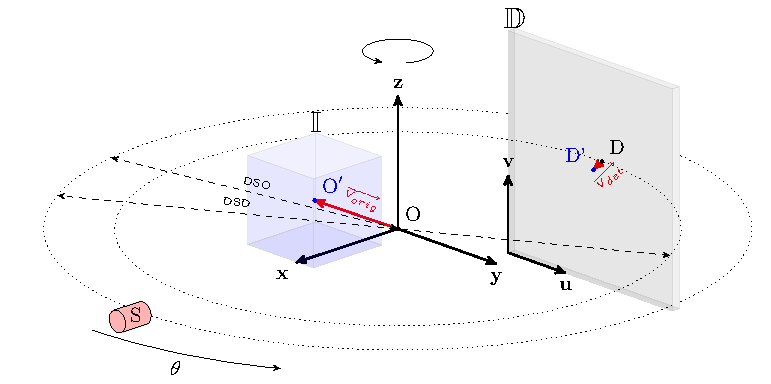
\includegraphics{GPUmethods/geometrytikz-figure0.pdf} 
\end{center}

\caption[Diagram of the geometry of TIGRE]{\label{fig:geometryTIGRE} Diagram of the geometric definition of a TIGRE reconstruction. Image, and detector offsets are supported, as well as any arbitrary size for the image and the detector, both total and pixel-wise.} 
\end{figure}

The geometric variables described above are used in the TIGRE Toolbox to perform the necessary operations for image reconstruction, as shown in code snippet \ref{cs:geometry}. It is worth mentioning that both $\overrightarrow{V_{det}}$, $\overrightarrow{V_{orig}}$, COR and the rotation of the detector are vectors that can be defined per projection angle $\theta$.
\FloatBarrier
\begin{lstlisting}[style=Matlab-editor,
basicstyle=\scriptsize,
caption= Geometry definition in TIGRE,
label={cs:geometry},
frame = single
]
%% Geometry structure definition.
% Distances
geo.DSD = 1536;                      	    % Distance Source Detector
geo.DSO = 1000;                     	    % Distance Source Origin
% Detector parameters
geo.nDetector=[512; 512];		    % number of pixels 
geo.dDetector=[0.8; 0.8]; 		    % size in mm of each pixel
geo.sDetector=geo.nDetector.*geo.dDetector; % total size of the detector in mm
geo.rotDetector=[0;0;0];                    % euler angles of the rotation 
% Image parameters
geo.nVoxel=[512;512;512];                   % number of voxels in the image
geo.sVoxel=[256;256;256];                   % total size of the image in mm
geo.dVoxel=geo.sVoxel./geo.nVoxel;          % size in mm of each voxel
% Offsets
geo.offOrigin  =[0; 0; 0];                  % V_orig
geo.offDetector=[0; 0];                     % V_det
geo.COR=0;                                  % Centre of Rotation offset

\end{lstlisting}

\subsection{Structure}

TIGRE has been designed to be modular, in order to facilitate prototyping with instant acceleration and to allow easy of the toolbox. The main building blocks are the projection ($A(x)$) and back projection ($A^T(b)$) operators. In the TIGRE Toolbox, these two blocks have been optimized for GPU computing using CUDA, as described in the beginning of this chapter. They lie in the lowest layer of the toolbox design and are constantly used by the other layers. The algorithms themselves lie in the topmost layer and are all coded in MATLAB, which provides the power and flexibility of a high-level language. To be able to communicate between the low-level, hardware-oriented CUDA and the high-level, design-oriented MATLAB, a set of the so-called \textit{MEX functions} are needed. The toolbox has been designed not to have any specific data types or classes. Instead, it comprises only the basic MATLAB types, such as matrices and structures.

The high level algorithms are designed to have multiple parameters and full customization. The only required parameters to all algorithms are the data, geometry, angles and number of iterations. Each algorithm has a series of tunable parameters. Generally every parameter affecting the algorithm can be set up to have a different value, allowing users that want to study algorithm behaviour full customization, but having default parameters in case the users want an easy-to use algorithm. Multiple algorithm initialization modes, angle ordering schemes and other features are also available. 

\begin{figure}
\begin{center}

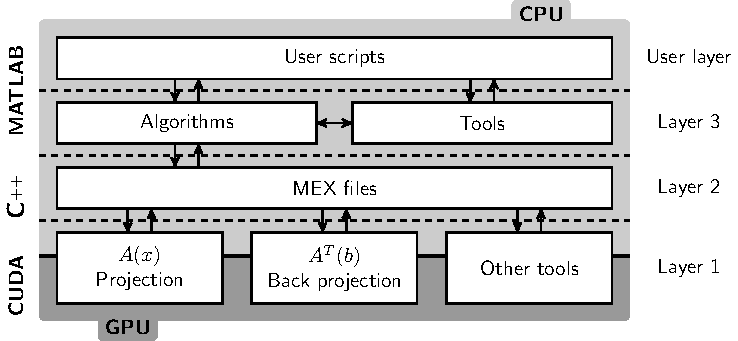
\includegraphics{GPUmethods/structureTIGRE-figure0.pdf} 
\end{center}

\caption[Diagram of the structure of the TIGRE toolbox]{\label{fig:structureTIGRE} Diagram of the structure on TIGRE toolbox.} 
\end{figure}

\subsubsection{Using TIGRE}
This code demonstrates the reconstruction of the RANDO head phantom (data obtained in the Christie Hospital, Manchester, UK) using three different algorithms with the geometry defined in code snippet \ref{cs:geometry}. The data set contains 360 equidistant projections. Once the data have been loaded using the code of snippet \ref{cs:randohead}, the results of figure \ref{fig:RANDOTIGRE} can be obtained without the need for any more code. Information about total computation time and computation time per iteration are shown. Only some of the possible optional parameters to the algorithms are shown in the snippet. The reader is referred to the published documentation for advanced options and for insight into their numerical ranges. 

\begin{lstlisting}[style=Matlab-editor,
basicstyle=\scriptsize,
caption= RANDO head data reconstruction,
label={cs:randohead},
frame = single
]
% Define Geometry & load data

% From the data, the projection angles (in radians) must have been read
angles= 0:359*pi/180; % as an example 

%% Reconstruct image with different algorithms
% FDK
imgFDK=FDK(data,geo,angles);
% CGLS
iterCGLS=15;
imgCGLS=CGLS(data,geo,angles,iterCGLS);
% OS-SART with multi-grid initialization
iterOSSART=70; 
imgOSSART=OS_SART(data,geo,angles,iterOSSART,'BlockSize',20,'Init','multigrid');

\end{lstlisting}





\begin{figure}
\centering
\begin{tikzpicture}

\node (A) {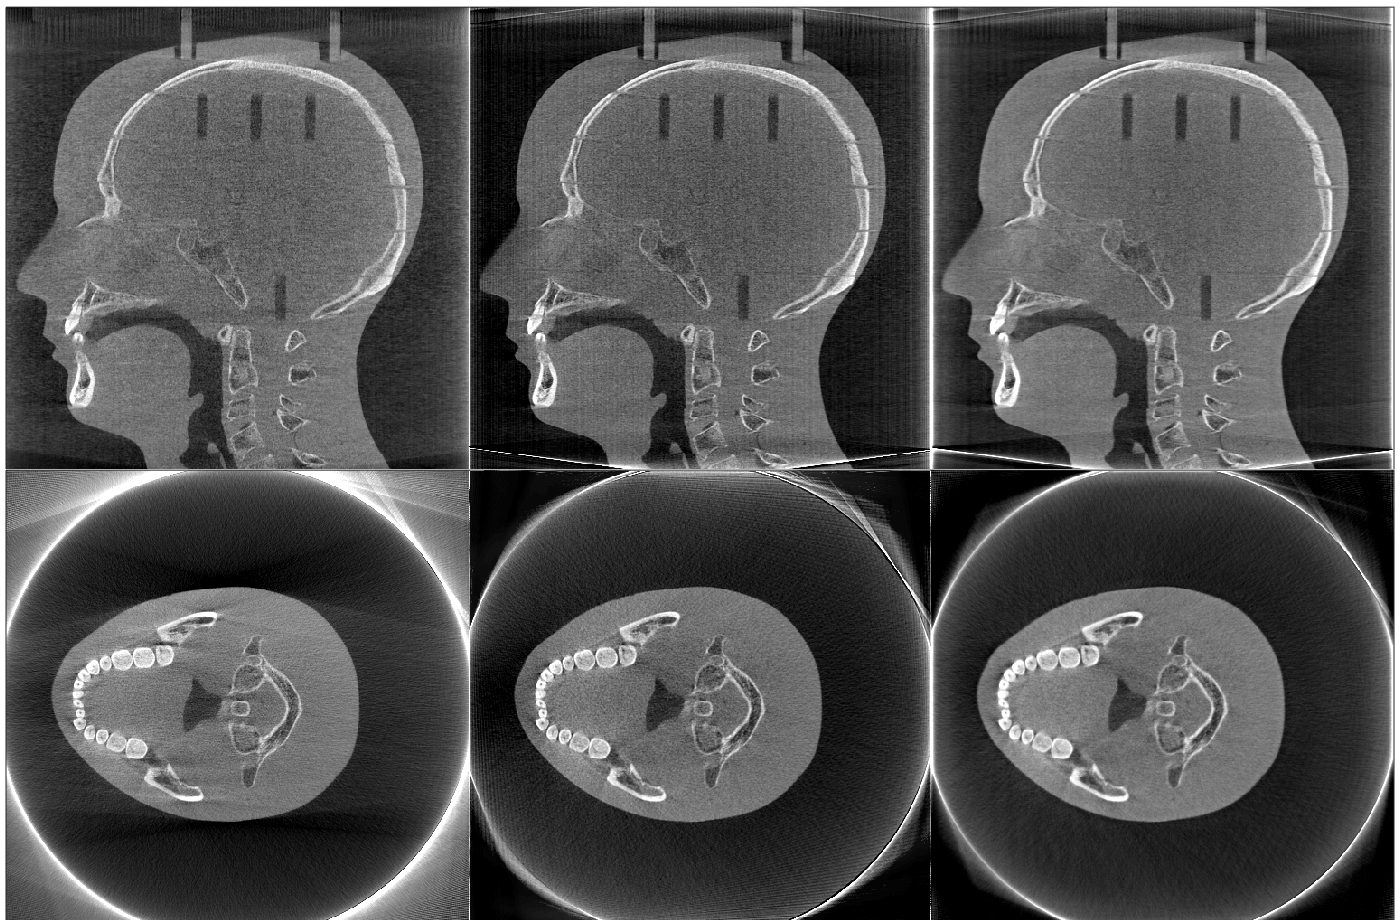
\includegraphics[width=0.98\textwidth]{GPUmethods/RANDO.png} };
\path (A.south west) -- (A.south east) node[pos=.175, below,align=center] {(a)\\ FDK \\14s total} node[pos=.5, below,align=center] {(b) \\OS-SART\\20m59s total\\31s per iteration} node[pos=.825, below,align=center] {(c)\\ CGLS \\ 6m8s total \\ 18s per iteration};
\end{tikzpicture}

\caption[RANDO head recosntructed in TIGRE using FDk,OS-SART and CGLS]{\label{fig:RANDOTIGRE} RANDO head phantom reconstructed with (a) FDK, (b) OS-SART 40 iterations and (c) CGLS 20 iterations, for 360 equidistant projections. The computational times are also shown.} 
\end{figure}



\subsubsection{Implementation of an algorithm in TIGRE}
To demonstrate the facility with which anyone can develop new algorithms using the
TIGRE toolbox, this section presents a side by side comparison of an algorithm definition and its TIGRE equivalent code, using the GPU accelerated features. For the
sake of brevity, the CGLS algorithm has been chosen.
In table \ref{tab:CGLSTIGRE} the definition of the CGLS iterations and the implementation in TIGRE
are shown. From the code snippet, it is worth highlighting the limited use of library related
functions, as one of the strengths of TIGRE for the developer point of view is the
easy to use Application Programming Interface (API). The only difference in the code
from a completely standard MATLAB script is the use of the function Ax() and Atb(),
the main building blocks of the toolbox. This allows anyone
with MATLAB code for solving image reconstruction to easily modify their code by just
changing the matrix-vector operations by TIGRE GPU functions. Note that the functions inside TIGRE do generally have more code than the one shown here, as several options and performance enhancing MATLAB tools are used.

\pagebreak


\begingroup
\captionof{table}{CGLS algorithm as definition, and implemented in TIGRE}\label{tab:CGLSTIGRE}
\endgroup
\begin{multicols}{2}
\begin{flalign*}
\label{eq:CGLSalgorithm}
%\begin{split}
&x_0=0; \; d_0=b; \; r_0=A^T b; p_0=r_0;&\\
&t_0=A r_0; \; \gamma_{k-1}=\left \| r_0 \right \|^2;&\\
&\textbf{for} \;k=1\; \textbf{to}\; k=\text{maxiter} &\\
&\;\;\;\; \alpha_k= \gamma_{k-1} / \left \| t_{k-1} \right \|^2 &\\
&\;\;\;\; x_k=x_{k-1}+\alpha_k t_{k-1}&\\
&\;\;\;\; d_k=d_{k-1}-\alpha_k t_{k-1}&\\
&\;\;\;\; r_k=A^Td_k &\\
&\;\;\;\; \gamma_k=\left \| r_{k} \right \|^2&\\
&\;\;\;\; \beta_k=  \gamma_{k} / \gamma_{k-1}&\\
&\;\;\;\; p_k=r_k+\beta_kp_{k-1} &\\
&\;\;\;\; t_k=Ap_k& \\
& \textbf{end}&
%\end{split}
\end{flalign*}
\columnbreak
\begin{lstlisting}[style=Matlab-editor,
basicstyle=\scriptsize,
label={cs:cgls},frame = single]
% Initialize variables
x=zeros(geo.nVoxel'); 
d=b;
r=Atb(b,geo,angles,'matched'); %TIGRE
p=r;
t=Ax(r,geo,angles); %TIGRE
gamma_1=norm(r(:));

% Loop until user defined maxiter
for k=1:maxiter
   alpha=gamma_1/norm(t(:));
   x=x+alpha*t;
   d=d-alpha*t;
   r=Atb(d,geo,angles,'matched');%TIGRE
   gamma=norm(r(:));
   beta=gamma/gamma_1;
   gamma_1=gamma;
   p=r+beta*p;
   t=Ax(p,geo,angles); %TIGRE  
end
% x is the solution.
\end{lstlisting}
\end{multicols}



\section{Summary}


In this chapter we have presented a MATLAB/CUDA toolbox for fast 3D X-ray image reconstruction. While the toolbox has reasonably good performance -- reducing to minutes an image reconstruction with complex iterative algorithms -- and a wide variety of tools, improvements are possible.

The projection and back projection operators have been fully implemented in the GPU, but the algorithms are fully in CPU so a memory management overhead exists because the data need to be introduced and extracted from the GPU twice per iteration. This design has been proposed in order to have the algorithms in a high-level language, as an algorithm implementation cycle in a low-level language like C++ is significantly longer than in MATLAB. As an estimate, if the algorithms were written in C++/CUDA directly, an improvement in computation time of up to 50\% could be achieved in some cases. However, this would increase the difficulty of adding new algorithms to the toolbox. The final decision was that the advantages of a high-level programming language for new algorithms are better than the possible benefits of doubling the speed, which is already reasonably good. 

Further improvements in the core GPU kernels of the toolbox would also be possible. While the speeds reached by this method are arguably state of the art, some improvements to the kernel structure to decrease even more memory latency and computational times have been proposed in the literature. It is impossible to know with certainty that any of the methods published will increase the speed of the code, partly because GPU architecture has changed over the past year massively, thus code may be faster in specific GPUs but slower in others, and partly because most of the published papers do not contain code to be benchmarked against, and use different geometric parameters each. Thompson and Lionheart\cite{thompson2014gpu} propose a method that exploits structure similarities and works if the cone angle is smaller than 45 degrees, that is the case of most commercial CBCT machines. The work in this thesis tries not to impose limitations on the possible geometries, but modifying the code to trigger the accelerated version proposed by Thompson and Lionheart is an interesting possibility. Chou \emph{et al}\cite{chou2011fast} claim speed-up by re-structuring the kernels to lauch multiple treads for multiple rays in parallel. While initial trials for replicating the multithreads in the early stages of the work in this thesis failed (as times where not changes) the projection operator has intensively been modified since then. This work has potential to accelerate up to 600\% the projection operation according to the article. Finally, the method proposed by Gao\cite{gao2012fast} claims significant speed-up over the ``naive'' Siddon's method, the code provided with their article shows slower execution for both the ``naive'' and accelerated versions than the code used in this work. Nevertheless, it would be worth implementing their approach.

The backprojection operator has been more optimized than the projection operation, using better techniques, thus speed-wise it is performing well. \color{red}{However, there are certainly faster methods, as TIGRE ranks between 5 and 7 in the RabbitCT\footnote{\href{https://www5.cs.fau.de/research/projects/rabbitct}{https://www5.cs.fau.de/research/projects/rabbitct}} benchmark.}\color{black}{} The RabbitCT benchmark is also recorded in different machines, thus some of the faster methods are due to multi-GPU parallelism exploits or just simply due to faster GPUs. That said, there is certainly room for improvement. 
Possibly the biggest improvement to the backprojection  would be the implementation of completely matched projection adjoint code, as it leads to better recosntruction\cite{6829349}. Thompson and Lionheart\cite{thompson2014gpu} propose a technique, so does Gao\cite{gao2012fast}.

Comparing the forward and back projection speeds to the ASTRA toolbox\cite{ASTRA},\color{red}{ TIGRE is 2 times slower at its worst}\color{black}{}. This can be easily explained by two factors. Firstly, the geometric options for CBCT are more flexible in TIGRE than in ASTRA, thus requiring more floating-point operations. Secondly, ASTRA implements an advanced ray splitting that increases memory latency in the GPU and that makes use of overlaps between X-ray paths at different angles\cite{Palenstijn2011250}. Adding all the discussed effects that would decrease the time performance, all algorithms run about 3 times more slowly in TIGRE than in ASTRA, which constitutes the state of the art. {Numerically, the differences between ASTRA and TIGRE are in absolute value of the order of $10^{-3}$, which is about 0.01\% in relative terms. This difference can be attributed to accumulated floating point errors due to different numerical approaches in the GPU code.}

 \color{red}{To speed up further the toolbox, a multi-GPU approach could also be taken. Currently, TIGRE does not support multi-GPU architectures.} \color{black}{} A further weakness of the toolbox is the small number of functions for data loading and post-processing. However, work will be continued, hopefully filling this gap in the near future. The single GPU limitation of TIGRE also limits the image size. Currently, 12GB is the maximum amount of memory on a GPU board, thus limiting the possible size of the images that can be reconstructed. Nevertheless, there is no problem to reconstruct a $1024^3$ image with most algorithms so the maximum image size is still big.

The TIGRE Toolbox has been designed with the objective of reducing the gap between image reconstruction research and the end users of tomographic images. While research in reconstruction creates new algorithms every year, end users only have access to FDK implementations. With these two groups in mind, the toolbox:
\begin{itemize}
\item has easy-to-use ``black box'' algorithms, making it extremely straightforward for researchers who are only interested in the quality of the images to test different algorithms without them requiring any knowledge of how the algorithms work;
\item has easy-to-use building blocks (projection and back projection operators) that allow algorithm developers to test new methods using a high-level programming language but with the performance of the lowest level, GPU languages.
\end{itemize}
The code is released as open source under a BSD 3-clause license, allowing anyone to download, test, modify and improve it. While the toolbox was originally designed for CBCT image reconstruction, an option for 3D parallel-beam CT reconstruction has also been included allowing for more geometries, e.g., synchrotron data. Further tweaking the geometry structure of the toolbox also permits 2D fan- and parallel-beam reconstructions.

% We enthusiastically encourage the submission of improvements, bug-fixes, demos, data and whatever else might help the community. Likewise, we encourage algorithm developers to submit their new algorithms to the toolbox, giving them visibility. Finally, we would like to encourage X-ray image end users to include data or descriptions of specific challenges they may have, allowing dialogue and hopefully leading to better ways of creating enhanced tomographic images. 

The minimum requirements to run the toolbox are strongly dependent on the image size desired, as memory is the strongest limiting factor both on the CPU and GPU side. Generally speaking, any NVIDIA GPU with a compute capability higher than 3.5 would be sufficient to reconstruct arbitrarily large images. We recommend having at least 3 times the desired image size in GPU memory and 8 times in RAM in the computer. As an example, for a $512^3$ image, 2GB of GPU memory and 6GB of computer RAM is the suggested minimum. The computing power (number of processors in the GPU and processor performance of the CPU) will have a strong effect on the speed of image reconstruction. 


%Projection:


%While there is potential for improvement, the speeds achieved with the code in developed are fast enough (see section \ref{sec:speed} for speed tests) for the intended purposes in this work.